\documentclass[10pt]{article}
\usepackage[vietnamese]{babel}
\usepackage[utf8]{inputenc}
\usepackage[T5]{fontenc}
\usepackage{caption}
\usepackage{amsmath}
\usepackage{amsfonts}
\usepackage{amssymb}
\usepackage[version=4]{mhchem}
\usepackage{stmaryrd}
\usepackage{graphicx}
\usepackage[export]{adjustbox}
\graphicspath{ {./images/} }
\usepackage{multirow}

\DeclareUnicodeCharacter{2020}{\ifmmode\dagger\else{$\dagger$}\fi}

\begin{document}
\captionsetup{singlelinecheck=false}
\section*{CHUONG \\
 1 CẤU TAO NGUYÊN TỬ}
\begin{table}[h]
\begin{center}
\captionsetup{labelformat=empty}
\caption{Bài 1. THÀNH PHẦN CỦA NGUYÊN TỬ}
\begin{tabular}{|l|l|l|l|l|l|l|}
\hline
1.1. $B$ & 1.2. $B$ & $1.3 . C$ & $1.6 . B$ & $1.7 . A$ & $1.9 . D$ & $1.10 . C$ \\
\hline
\end{tabular}
\end{center}
\end{table}

1.4.

\begin{center}
\begin{tabular}{|l|l|l|l|l|l|l|}
\hline
Nguyên tố & Kí hiệu & Z & Số e & Số p & Số n & Số khối \\
\hline
Carbon & C & 6 & 6 & 6 & 6 & 12 \\
\hline
Nitrogen & N & 7 & 7 & 7 & 7 & 14 \\
\hline
Oxygen & O & 8 & 8 & 8 & 8 & 16 \\
\hline
Sodium & Na & 11 & 11 & 11 & 12 & 23 \\
\hline
\end{tabular}
\end{center}

1.5. - Có thể tạo ra chùm electron bằng cách phóng điện với hiệu điện thế rất cao (khoảng 10000 V ) qua không khí loãng (khoảng $1,3 \cdot 10^{-6}$ bar).

\begin{itemize}
  \item Khối lượng của electron bằng $9,109 \cdot 10^{-31}(\mathrm{~kg})$.
  \item Điện tích electron bằng $-1,602 \cdot 10^{-19}(\mathrm{C})$.\\
1.8. $1 \mathrm{amu}=1,661 \cdot 10^{-27} \mathrm{~kg}$.
\end{itemize}

Khối lượng của nguyên tử oxygen theo amu:

$$
\frac{26,5595}{1,661} \approx 15,99(\mathrm{amu})
$$

Khối lượng mol của oxygen là $15,99 \mathrm{~g} / \mathrm{mol}$.\\
1.11. a) Nguyên tử trung hoà về điện nên $p=e$.

Theo bài ra ta có: $2 p+n=40$ và $2 p-n=12$\\
$\Rightarrow p=e=13$ và $n=14$\\
b) Số khối của X là: $13+14=27$.\\
1.12. Số electron $=13$, khối lượng $1 \mathrm{p}=1,673 \cdot 10^{-24}(\mathrm{~g})$.

Số mol nhôm $=1 \mathrm{~mol}$\\
$\Rightarrow$ Khối lượng proton là: $13 \cdot 1,673 \cdot 10^{-24} \cdot 6,022.10^{23}=13,0972(\mathrm{~g})$.\\
Khối lượng neutron là: $14 \cdot 1,675.10^{-24} \cdot 6,022 \cdot 10^{23}=14,1216(\mathrm{~g})$.\\
Khối lượng electron là: $13 \cdot 9,109 \cdot 10^{-28} \cdot 6,022 \cdot 10^{23}=7,131.10^{-3}(\mathrm{~g})$.\\
1.13. Trong nguyên tử B : số $\mathrm{p}=$ số $\mathrm{e}=5$; số $\mathrm{n}=6$.

Khối lượng hạt nhân nguyên tử B là: $18,415 \cdot 10^{-27}(\mathrm{~kg})$.\\
Khối lượng nguyên tử B là: $18,420 \cdot 10^{-27}(\mathrm{~kg})$.\\
Tỉ số khối lượng nguyên tử : khối lượng hạt nhân $=1,000272$.\\
$\Rightarrow$ Khối lượng nguyên tử tập trung chủ yếu ở hạt nhân.

\section*{Bài 2. NGUYÊN TỐ HOÁ HỌC}
\begin{center}
\begin{tabular}{|l|l|l|l|l|}
\hline
2.1. C & $2.2 . \mathrm{A}$ & $2.3 . \mathrm{C}$ & $2.4 . \mathrm{A}$ & $2.5 . \mathrm{B}$ \\
\hline
2.6. D & $2.7 . \mathrm{D}$ & $2.8 . \mathrm{D}$ & $2.9 . \mathrm{A}$ & $2.10 . \mathrm{B}$ \\
\hline
\end{tabular}
\end{center}

2.7. Đồng vị ${ }^{14} \mathrm{~N}$ kết hợp với ( ${ }^{16} \mathrm{O},{ }^{16} \mathrm{O}$ ); ( ${ }^{17} \mathrm{O},{ }^{17} \mathrm{O}$ ); $\left({ }^{18} \mathrm{O},{ }^{18} \mathrm{O}\right) ;\left({ }^{16} \mathrm{O},{ }^{17} \mathrm{O}\right)$; ( ${ }^{16} \mathrm{O},{ }^{18} \mathrm{O}$ ); ( ${ }^{17} \mathrm{O},{ }^{18} \mathrm{O}$ ) được 6 hợp chất $\mathrm{NO}_{2}$.\\
Tương tự, đồng vị ${ }^{15} \mathrm{~N}$ kết hợp với 6 cặp đồng vị O như trên được 6 hợp chất $\mathrm{NO}_{2}$ nữa (chọn D ).\\
2.11. Gọi $\%{ }_{5}^{10} \mathrm{~B}$ là $\mathrm{x}, \%{ }_{5}^{11} \mathrm{~B}=100-\mathrm{x}$.

Ta có: $10 \mathrm{x}+11(100-\mathrm{x})=1081$\\
$\Rightarrow \mathrm{x}=19$ và $100-\mathrm{x}=81$.\\
Vậy phần trăm số nguyên tử ${ }^{10} \mathrm{~B}$ là $19 \%$ và ${ }^{11} \mathrm{~B}$ là $81 \%$.\\
2.12. Gọi hàm lượng ${ }_{27}^{58} \mathrm{Co}$ và ${ }_{27}^{60} \mathrm{Co}$ lần lượt là x và y .

Ta có: $58 \mathrm{x}+(59 \cdot 0,98)+60 \mathrm{y}=58,982$\\
và $\mathrm{x}+\mathrm{y}=1-0,98=0,02$

Giải hệ (I) và (II), ta được: $\mathrm{y}=0,001$.\\
$\Rightarrow$ Hàm lượng \% của đồng vị phóng xạ Co-60 là $0,1 \%$.

\section*{Bài 3. CẤU TRÚC LỚP VỎ ELECTRON NGUYÊN TƯ}
\begin{center}
\begin{tabular}{|l|l|l|l|l|l|}
\hline
3.1. C & 3.2. C & $3.3 . \mathrm{B}$ & $3.4 . \mathrm{D}$ & $3.5 . \mathrm{B}$ & $3.6 . \mathrm{C}$ \\
\hline
3.7. B & $3.8 . \mathrm{A}$ & $3.9 . \mathrm{B}$ & $3.10 . \mathrm{A}$ & $3.11 . \mathrm{D}$ & $3.12 . \mathrm{B}$ \\
\hline
3.13. C & $3.14 . \mathrm{D}$ & $3.15 . \mathrm{D}$ & $3.16 . \mathrm{C}$ & $3.17 . \mathrm{D}$ & $3.18 . \mathrm{B}$ \\
\hline
\end{tabular}
\end{center}

3.19. Cách sắp xếp electron trong orbital s bằng ô lượng tử: $\square$ $\uparrow \square \uparrow \downarrow$.\\
3.20. Trường hợp orbital p có chứa 2 e :

\begin{figure}[h]
\begin{center}
  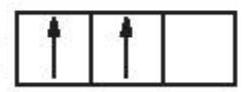
\includegraphics[width=\textwidth]{2025_10_23_ee735750217b2aca435cg-03(1)}
\captionsetup{labelformat=empty}
\caption{(1)}
\end{center}
\end{figure}

\begin{figure}[h]
\begin{center}
  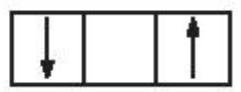
\includegraphics[width=\textwidth]{2025_10_23_ee735750217b2aca435cg-03(3)}
\captionsetup{labelformat=empty}
\caption{(2)}
\end{center}
\end{figure}

\begin{figure}[h]
\begin{center}
  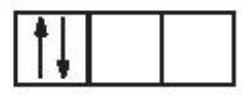
\includegraphics[width=\textwidth]{2025_10_23_ee735750217b2aca435cg-03}
\captionsetup{labelformat=empty}
\caption{(3)}
\end{center}
\end{figure}

\begin{figure}[h]
\begin{center}
  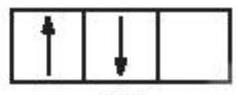
\includegraphics[width=\textwidth]{2025_10_23_ee735750217b2aca435cg-03(4)}
\captionsetup{labelformat=empty}
\caption{(4)}
\end{center}
\end{figure}

\begin{figure}[h]
\begin{center}
  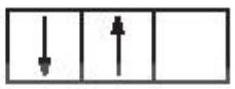
\includegraphics[width=\textwidth]{2025_10_23_ee735750217b2aca435cg-03(6)}
\captionsetup{labelformat=empty}
\caption{(5)}
\end{center}
\end{figure}

\begin{figure}[h]
\begin{center}
  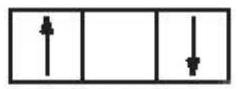
\includegraphics[width=\textwidth]{2025_10_23_ee735750217b2aca435cg-03(5)}
\captionsetup{labelformat=empty}
\caption{(6)}
\end{center}
\end{figure}

\begin{figure}[h]
\begin{center}
  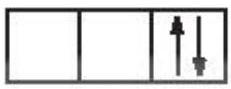
\includegraphics[width=\textwidth]{2025_10_23_ee735750217b2aca435cg-03(7)}
\captionsetup{labelformat=empty}
\caption{(7)}
\end{center}
\end{figure}

\begin{figure}[h]
\begin{center}
  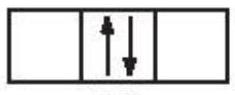
\includegraphics[width=\textwidth]{2025_10_23_ee735750217b2aca435cg-03(2)}
\captionsetup{labelformat=empty}
\caption{(8)}
\end{center}
\end{figure}

Chỉ có cách (1) tuân theo quy tắc Hund.\\
3.21. Mối quan hệ về năng lượng:

\begin{itemize}
  \item Khi chuyển động trong nguyên tử các electron có thể chiếm những mức năng lượng khác nhau đặc trưng cho trạng thái chuyển động của nó. Những electron chuyển động gần hạt nhân hơn, chiếm những mức năng lượng thấp hơn, tức là ở trạng thái bền hơn những electron chuyển động ở xa hạt nhân có năng lượng cao hơn. Mức năng lượng tăng dần theo $\mathrm{AO}: \mathrm{s}<\mathrm{p}<\mathrm{d}<\mathrm{f}$.
  \item Các electron thuộc cùng một lớp có mức năng lượng gần bằng nhau. Những electron ở lớp bên trong có năng lượng thấp hơn và liên kết với hạt nhân bền chặt hơn so với những electron ở lớp ngoài. Mức năng lượng tăng dần theo lớp electron: $\mathrm{K}<\mathrm{L}<\mathrm{M}<\mathrm{N}<\mathrm{O}<\ldots$
  \item Các electron trên cùng một phân lớp có năng lượng bằng nhau.\\
3.22. Tổng số electron tối đa chứa trong:\\
a) Phân lớp $\mathrm{p}=6(3 \mathrm{AO})$;\\
b) Phân lớp $\mathrm{d}=10(5 \mathrm{AO})$.\\
c) Lớp $\mathrm{K}=2(1 \mathrm{AO})$;\\
d) Lớp $M=18(9 \mathrm{AO})$.\\
3.23. - Nguyên tử X có cấu hình electron: $1 \mathrm{~s}^{2} 2 \mathrm{~s}^{2} 2 \mathrm{p}^{6} 3 \mathrm{~s}^{2}$.\\
$X$ nhường đi 2 electron: $X \rightarrow X^{2+}+2 e$
\end{itemize}

Cấu hình e của ion $\mathrm{X}^{2+}$ là $1 \mathrm{~s}^{2} 2 \mathrm{~s}^{2} 2 \mathrm{p}^{6}$.

\begin{itemize}
  \item Nguyên tử Y có cấu hình e : $1 \mathrm{~s}^{2} 2 \mathrm{~s}^{2} 2 \mathrm{p}^{6} 3 \mathrm{~s}^{2} 3 \mathrm{p}^{5}$.
\end{itemize}

Y nhận thêm 1 electron: $\mathrm{Y}+\mathrm{e} \rightarrow \mathrm{Y}^{-}$\\
Cấu hình e của ion $\mathrm{Y}^{-}$là $1 \mathrm{~s}^{2} 2 \mathrm{~s}^{2} 2 \mathrm{p}^{6} 3 \mathrm{~s}^{2} 3 \mathrm{p}^{6}$.

\begin{itemize}
  \item Cấu hình electron của ion $\mathrm{X}^{2+}$ giống khí hiếm Ne ;
\end{itemize}

Cấu hình electron của ion $\mathrm{Y}^{-}$giống với cấu hình electron của khí hiếm Ar .\\
3.24. Cấu hình electron của nguyên tử:\\
$-Z=9\left(1 \mathrm{~s}^{2} 2 \mathrm{~s}^{2} 2 \mathrm{p}^{5}\right): \quad \uparrow \downarrow \square|\uparrow| \downarrow \mid$, nguyên tử có 7 electron hoá trị, dễ thu electron, là phi kim.

$-\mathrm{Z}=14\left(1 \mathrm{~s}^{2} 2 \mathrm{~s}^{2} 2 \mathrm{p}^{6} 3 \mathrm{~s}^{2} 3 \mathrm{p}^{2}\right): \quad$ † $\downarrow$ | | $\square|\downarrow| \downarrow|\downarrow| \uparrow |$\begin{tabular}{|l|l|l|}
\hline
 &  &  \\
\hline
 &  &  \\
\hline
\end{tabular} có 4 electron hoá trị nên có thể thu electron hoặc nhường electron, là phi kim.

$-Z=21\left(1 s^{2} 2 s^{2} 2 p^{6} 3 s^{2} 3 p^{6} 4 s^{2} 3 d^{1}\right):$

\begin{center}
\begin{tabular}{|l|l|l|l|l|l|l|l|l|l|l|l|l|l|l|l|}
\hline
$\uparrow$ & 11 & $\uparrow \downarrow$ & $\uparrow \downarrow$ & $\uparrow \downarrow$ & $\square$ & $\dagger 1$ & | $\downarrow$ & $\uparrow \downarrow$ & $\uparrow$ & $\uparrow$ & $\square$ &  & \multicolumn{2}{|c|}{} & $\square$ \\
\hline
\end{tabular}
\end{center}

nguyên tử có 3 electron hoá trị, dễ nhường electron, là kim loại.\\
3.25. a) Coi tổng số hạt trong $[M]$ là $x$ và $[X]$ là $y$

Theo bài ra ta có: $4 x+3 y=214$\\
và


\begin{equation*}
4 x-3 y=106 \tag{I}
\end{equation*}


Giải hệ (I) và (II), ta được: $\mathrm{x}=40$ và $\mathrm{y}=18$.\\
$2 \mathrm{p}_{\mathrm{M}}+\mathrm{n}_{\mathrm{M}}=40$ với $\mathrm{l} \leq \frac{\mathrm{n}_{\mathrm{M}}}{\mathrm{p}_{\mathrm{M}}} \leq 1,5$ và $\mathrm{p}_{\mathrm{M}}<20$ nên $\mathrm{p}_{\mathrm{M}}=13$ và $\mathrm{n}_{\mathrm{M}}=14$\\
$\Rightarrow \mathrm{M}$ là ${ }_{13} \mathrm{Al}$.\\
$2 p_{X}+n_{X}=18$ với $l \leq \frac{n_{X}}{p_{X}} \leq 1,5$ và $p_{X}<9$ nên $p_{X}=6$ và $n_{X}=6$\\
$\Rightarrow \mathrm{X}$ là 6 C .\\
Công thức hoá học của A là $\mathrm{Al}_{4} \mathrm{C}_{3}$.\\
b) Cấu hình electron: ${ }_{13} \mathrm{Al}\left(1 s^{2} 2 s^{2} 2 p^{6} 3 s^{2} 3 p^{1}\right)$ và $6 \mathrm{C}\left(1 s^{2} 2 s^{2} 2 p^{2}\right)$.

\section*{Bài 4. ÔN TẬP CHƯƠNG 1}
\begin{center}
\begin{tabular}{|l|l|l|l|l|l|l|}
\hline
4.1. B & 4.2. C & 4.3. A & 4.4. C & 4.5. C & 4.6. A & 4.7. B \\
\hline
4.8. C & 4.9. B & 4.10. C & 4.11. D & 4.12. A & 4.15. D & 4.16. A \\
\hline
\end{tabular}
\end{center}

4.13. Cấu hình electron theo ô orbital:\\
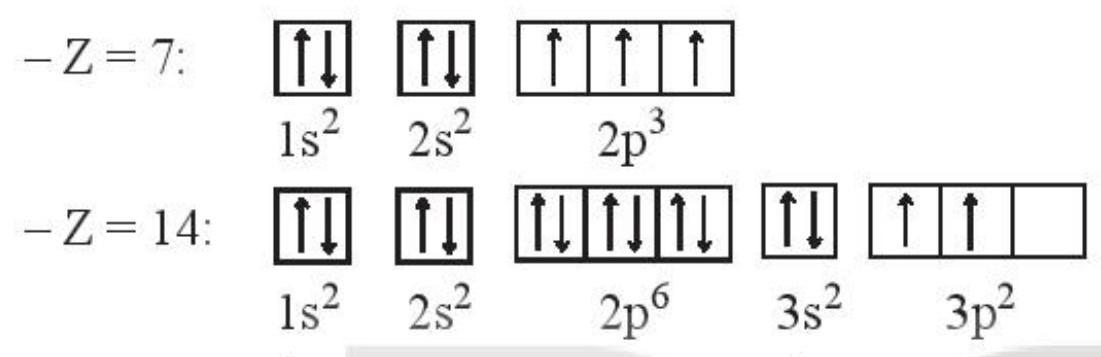
\includegraphics[max width=\textwidth, center]{2025_10_23_ee735750217b2aca435cg-05}

Giải thích: cấu hình electron được viết tuân theo nguyên lí vững bền, nguyên lí Pauli và phần $2 \mathrm{p}^{3}, 3 \mathrm{p}^{2}$ tuân theo quy tắc Hund.

\begin{center}
\begin{tabular}{|l|l|l|l|l|l|l|l|l|l|}
\hline
\multirow[t]{2}{*}{$-\mathrm{Z}=21$ :} & $\dagger 1$ & $\uparrow \downarrow$ & | $\downarrow \uparrow \downarrow \mid \uparrow \downarrow$ & [1] & | | | | | | | & | 1 & $\uparrow$ &  &  \\
\hline
 & $1 \mathrm{~s}^{2}$ & $2 \mathrm{~s}^{2}$ & $2 \mathrm{p}^{6}$ & $3 \mathrm{~s}^{2}$ & $3 \mathrm{p}^{6}$ & $4 \mathrm{~s}^{2}$ &  & $3 \mathrm{~d}^{1}$ &  \\
\hline
\end{tabular}
\end{center}

Giải thích: cấu hình electron có phân lớp $4 \mathrm{~s}^{2}$ đặt trước phân lớp $3 \mathrm{~d}^{1}$ là tuân theo nguyên lí vững bền.\\
4.14. Cấu hình electron nguyên tử của các nguyên tố\\
$-Z=9\left(1 s^{2} 2 s^{2} 2 p^{5}\right) \Rightarrow$ lớp ngoài cùng có $7 e \Rightarrow$ phi kim.\\
$-\mathrm{Z}=16\left([\mathrm{Ne}] 3 \mathrm{~s}^{2} 3 \mathrm{p}^{4}\right) \Rightarrow$ lớp ngoài cùng có $6 \mathrm{e} \Rightarrow$ phi kim.\\
$-Z=18\left(1 \mathrm{~s}^{2} 2 \mathrm{~s}^{2} 2 \mathrm{p}^{6} 3 \mathrm{~s}^{2} 3 \mathrm{p}^{6}\right) \Rightarrow$ lớp ngoài cùng có $8 \mathrm{e} \Rightarrow$ khí hiếm.\\
$-\mathrm{Z}=20$ ( $[\mathrm{Ar}] 4 \mathrm{~s}^{2}$ ) $\Rightarrow$ lớp ngoài cùng có $2 \mathrm{e} \Rightarrow$ kim loại.\\
$-\mathrm{Z}=29\left([\mathrm{Ar}] 3 \mathrm{~d}^{10} 4 \mathrm{~s}^{1}\right) \Rightarrow$ lớp ngoài cùng có $1 \mathrm{e} \Rightarrow$ kim loại.\\
Chư ý: khi đến gần cấu hình bão hoà $\mathrm{d}^{10} ; \mathrm{f}^{14}$ hay cấu hình nửa bão hoà $\mathrm{d}^{5}, \mathrm{f}^{7}$ (cấu hình bền) thì nguyên tử sẽ đạt ngay cấu hình này, mặc dù phân lớp trước chưa đầy đủ electron.\\
4.17. Tổng các hạt cơ bản của $\mathrm{X}: \mathrm{p}+\mathrm{e}+\mathrm{n}=155$ hay $2 \mathrm{p}+\mathrm{n}=155$

Hạt mang điện là $p+e$ và không mang điện là $n$ nên $2 p-n=33$

Giải hệ (I) và (II), ta được: $\mathrm{p}=47$ và $\mathrm{n}=61$\\
$\Rightarrow$ số khối của $\mathrm{X}=108 \Rightarrow \mathrm{X}$ là silver $\left({ }_{47}^{108} \mathrm{Ag}\right)$.\\
4.18. a) Tổng các hạt cơ bản của $X: p+e+n=82$ hay $2 p+n=82$

Hiệu số hạt mang điện và không mang điện: $2 p-n=22$

Giải hệ (I) và (II), ta được: $\mathrm{p}=26$ và $\mathrm{n}=30$.\\
Nguyên tố $X$ có $Z_{X}=26, A x=26+30=56$ nên có kí hiệu nguyên tử ${ }_{26}^{56} X$.\\
b) Ion $\mathrm{X}^{2+}$ có $\mathrm{p}=26, \mathrm{n}=30, \mathrm{e}=\mathrm{p}-2=24$.

Cấu hình electron của $\mathrm{X}^{2+}: 1 \mathrm{~s}^{2} 2 \mathrm{~s}^{2} 2 \mathrm{p}^{6} 3 \mathrm{~s}^{2} 3 \mathrm{p}^{6} 3 \mathrm{~d}^{6}$.\\
4.19. a) Cấu hình electron của $A$ và $B$ có dạng:\\
$[\mathrm{Ne}] 3 \mathrm{~s}^{2} 3 \mathrm{p}^{6} 3 \mathrm{~d}^{\mathrm{x}} 4 \mathrm{~s}^{\mathrm{y}}(0 \leq \mathrm{x} \leq 10 ; 1 \leq \mathrm{y} \leq 2)$.

\begin{itemize}
  \item Nếu $\mathrm{y}=1$ thì cấu hình của $\mathrm{A}^{2+}$ là : $[\mathrm{Ne}] 3 \mathrm{~s}^{2} 3 \mathrm{p}^{6} 3 \mathrm{~d}^{\mathrm{x}-1}$
\end{itemize}

Khi đó có : $2+6+x-1=17 \Rightarrow x=10$.\\
Cấu hình electron của A là: $[\mathrm{Ar}] 3 \mathrm{~d}^{10} 4 \mathrm{~s}^{1} . \mathrm{A}$ là ${ }_{29} \mathrm{Cu}$.

\begin{itemize}
  \item Nếu $\mathrm{y}=2$ thì cấu hình của $\mathrm{A}^{2+}$ là : $[\mathrm{Ne}] 3 \mathrm{~s}^{2} 3 \mathrm{p}^{6} 3 \mathrm{~d}^{\mathrm{x}}$.
\end{itemize}

Khi đó có : $2+6+x=17 \Rightarrow x=9$\\
Cấu hình electron của A là: $[\mathrm{Ar}] 3 \mathrm{~d}^{9} 4 \mathrm{~s}^{2}$ (không bền vững).\\
Xét tương tự với B :

\begin{itemize}
  \item Nếu $\mathrm{y}=1$ thì cấu hình electron của B là $[\mathrm{Ar}] 3 \mathrm{~d}^{7} 4 \mathrm{~s}^{1}$ (không hợp lí).
  \item Nếu $y=2$ thì cấu hình electron của $B$ là $[\mathrm{Ar}] 3 \mathrm{~d}^{6} 4 \mathrm{~s}^{2}$. B là 26 Fe .\\
b) Số proton trong $\mathrm{Y}=\frac{87-26-29}{2}=16 . \mathrm{Y}$ là 16 S .
\end{itemize}

Quặng X có công thức là $\mathrm{CuFeS}_{2}$.

\section*{Bài 5. CẤU TẠO CỦA BẢNG TUẦN HOÀN CÁC NGUYÊN TỐ HOÁ HỌC}
\begin{center}
\begin{tabular}{|l|l|l|l|l|}
\hline
5.1. B & 5.2. D & $5.3 . \mathrm{B}$ & $5.4 . \mathrm{A}$ & $5.5 . \mathrm{C}$ \\
\hline
5.6. C & $5.7 . \mathrm{A}$ & $5.8 . \mathrm{C}$ & $5.9 . \mathrm{D}$ & $5.10 . \mathrm{B}$ \\
\hline
\end{tabular}
\end{center}

5.11. - Nguyên tử X có 11 electron và 1 electron lớp ngoài cùng nên ở ô số 11 , chu kì 3 , nhóm IA.

\begin{itemize}
  \item Nguyên tử Y có 7 electron và 5 electron lớp ngoài cùng nên ở ô số 7 , chu kì 2 , nhóm VA.
  \item Nguyên tử Z có 19 electron và 1 electron lớp ngoài cùng nên ở ô số 19 , chu kì 4, nhóm IA.\\
5.12. Nguyên tử $\mathrm{X}+1 \mathrm{e} \rightarrow$ anion $\mathrm{X}^{-}$\\
$\Rightarrow$ electron lớp ngoài cùng của X là $3 \mathrm{p}^{5} . \mathrm{X}$ là ${ }_{17} \mathrm{Cl}$.\\
Nguyên tử $\mathrm{Y} \rightarrow$ cation $\mathrm{Y}^{2+}+2 \mathrm{e}$\\
$\Rightarrow$ electron lớp ngoài cùng của Y là $4 \mathrm{~s}^{2} . \mathrm{Y}$ là Ca .\\
Vị trí trong bảng tuần hoàn: Cl ở ô số 17 , chu kì 3 , nhóm VIIA; Ca ở ô số 20 , chu kì 4 , nhóm IIA.\\
5.13. Nguyên tử $\mathrm{M} \rightarrow$ cation $\mathrm{M}^{3+}+3 \mathrm{e}$\\
$\Rightarrow$ electron lớp ngoài cùng của M là $3 \mathrm{~s}^{2} 3 \mathrm{p}^{1}$. M là 13 Al .\\
Nguyên tử $\mathrm{Y}+2 \mathrm{e} \rightarrow$ anion $\mathrm{Y}^{2-}$\\
$\Rightarrow$ electron lớp ngoài cùng của Y là $2 \mathrm{p}^{4}$. Y là 8 O .\\
Vị trí trong bảng tuần hoàn: Al ở ô số 13 , chu kì 3 , nhóm IIIA; O ở ô số 8 , chu kì 2, nhóm VIA.\\
5.14. Nguyên tố có $Z=26$ có cấu hình electron $[\mathrm{Ar}] 3 \mathrm{~d}^{6} 4 \mathrm{~s}^{2}$.
\end{itemize}

Vị trí trong bảng tuần hoàn: $Z$ ở ô số 26 , chu kì 4 , nhóm VIIIB.\\
5.15. Ta có: $\mathrm{p}+\mathrm{e}+\mathrm{n}=18$ hay $2 \mathrm{p}+\mathrm{n}=18$\\
$\Rightarrow \mathrm{p}<9 \Rightarrow \mathrm{X}$ thuộc chu kì 2 .

Với $\mathrm{p} \leq \mathrm{n}=18-2 \mathrm{p} \leq 1,33 \mathrm{p}$ nên $5,4 \leq \mathrm{p} \leq 6 \Rightarrow \mathrm{p}=6$.\\
X là C (carbon).\\
Nguyên tố C có số thứ tự 6 nằm ở chu kì 2 , nhóm IVA trong bảng tuần hoàn.\\
5.16. Số electron trong cation $=$ Số electron trong anion $=\frac{20}{2}=10$.

Có 3 trường hợp, $\mathrm{Al}^{3+}$ và $\mathrm{N}^{3-} ; \mathrm{Mg}^{2+}$ và $\mathrm{O}^{2-} ; \mathrm{Na}^{+}$và $\mathrm{F}^{-}$.\\
$\mathrm{N}^{3-}$ và $\mathrm{O}^{2-}$ không thoả mãn mức oxi hoá duy nhất (ví dụ: $\mathrm{N}^{+2}$ trong NO hay $\mathrm{O}^{2+}$ trong $\mathrm{F}_{2} \mathrm{O}$ ).\\
Vậy, $X$ là $N a$ ở ô số 11 , chu kì 3 , nhóm $I A$ và $Y$ là $F$ ở ô số 9 , chu kì 2 , nhóm VIIA của bảng tuần hoàn.\\
5.17. Số $\mathrm{p}=$ số e nên $2 \mathrm{p}+\mathrm{n}=34$ và $2 \mathrm{p}-\mathrm{n}=10 \Rightarrow \mathrm{p}=11$. R là 11 Na .

Vị trí trong bảng tuần hoàn của R : ô số 11 , chu kì 3 , nhóm IA .\\
5.18. Cùng nhóm A và ở hai chu kì kế tiếp với tổng $\mathrm{Z}=32$ thì số proton của hai nguyên tử chênh nhau 8 đơn vị. Tức là $p+p+8=32 \Rightarrow p=12$.\\
Vị trí trong bảng tuần hoàn của $\mathrm{A}, \mathrm{B}$ : ô số 12 và 20 , chu kì 3 và 4 , cùng nhóm IIA.

\section*{Bài 6. XU HƯỚNG BIẾN ĐỔI MỘT SỐ TÍNH CHẤT CỦA NGUYÊN TỬ CÁC NGUYÊN TỐ TRONG MỘT CHU Kİ VÀ TRONG MỘT NHÓM}
\begin{center}
\begin{tabular}{|l|l|l|l|l|l|}
\hline
$6.1 . \mathrm{B}$ & $6.2 . \mathrm{B}$ & $6.3 . \mathrm{D}$ & $6.4 . \mathrm{C}$ & $6.5 . \mathrm{B}$ & $6.6 . \mathrm{C}$ \\
\hline
$6.7 . \mathrm{A}$ & $6.8 . \mathrm{A}$ & $6.9 . \mathrm{C}$ & $6.10 . \mathrm{A}$ & $6.11 . \mathrm{D}$ & $6.12 . \mathrm{B}$ \\
\hline
$6.13 . \mathrm{C}$ & $6.14 . \mathrm{D}$ & $6.15 . \mathrm{B}$ & $6.16 . \mathrm{D}$ &  &  \\
\hline
\end{tabular}
\end{center}

6.17. - Sự giống nhau: trong cùng nhóm, các nguyên tử của nguyên tố nhóm A và B đều có số electron hoá trị bằng nhau nên có hoá trị cao nhất bằng nhau.

\begin{itemize}
  \item Sự khác nhau: số electron lớp ngoài cùng và cấu hình electron của các nguyên tố nhóm A và B không giống nhau nên tính chất vật lí, hoá học của chúng cũng khác nhau.\\
Ví dự: Cấu hình electron: 17 Cl : $[\mathrm{Ne}] 3 \mathrm{~s}^{2} 3 \mathrm{p}^{5}$ và 25 Mn : $[\mathrm{Ar}] 3 \mathrm{~d}^{5} 4 \mathrm{~s}^{2}$.
  \item Cl và Mn đều có 7 electron hoá trị nên đều có hoá trị cao nhất là 7 và số oxi hoá dương cao nhất là +7 .
  \item 7 electron hoá trị của Cl là electron $\mathrm{s}, \mathrm{p}$ còn 7 electron hoá trị của Mn là electron $\mathrm{s}, \mathrm{d}$.
  \item Nguyên tử Cl có 7 electron lớp ngoài cùng, nguyên tử Mn chỉ có 2 electron lớp ngoài cùng.
  \item Nguyên tố chlorine là phi kim điển hình còn nguyên tố manganese là kim loại chuyển tiếp.\\
6.18. a) Nguyên tử $\mathrm{X}, \mathrm{Y}$ đều có 5 electron hoá trị nên chúng ở cùng nhóm V .
\end{itemize}

Nguyên tử X có 5 electron lớp ngoài cùng, là nguyên tố p , thuộc nhóm VA.\\
Nguyên tử $Y$ có 5 electron ở lớp ngoài cùng và lớp sát ngoài cùng, là nguyên tố $d$, thuộc nhóm VB.\\
b) Nguyên tử $X$ có $n=3$ và nguyên tử $Y$ có $n=4$ nên $X$ thuộc chu kì 3 còn $Y$ thuộc chu kì 4 , chúng cách nhau 8 nguyên tố.\\
6.19. Liên hệ giữa các nguyên tố đó trong bảng tuần hoàn được mô tả trong bảng sau:

\begin{center}
\begin{tabular}{|l|l|l|l|l|}
\hline
 &  &  &  & 7 N \\
\hline
 & 12 Mg &  & 14 Si &  \\
\hline
19 K &  &  &  &  \\
\hline
\end{tabular}
\end{center}

Bán kính nguyên tử: $\mathrm{K}>\mathrm{Mg}, \mathrm{Si}>\mathrm{N}$.\\
Theo chu kì, bán kính nguyên tử giảm từ trái qua phải: $\mathrm{Mg}>\mathrm{Si}$.\\
Thứ tự giảm dần bán kính nguyên tử: $\mathrm{K}>\mathrm{Mg}>\mathrm{Si}>\mathrm{N}$.\\
6.20. Liên hệ giữa các nguyên tố đó trong bảng tuần hoàn được mô tả trong bảng sau:

\begin{center}
\begin{tabular}{|l|l|l|l|l|}
\hline
 &  &  &  & ${ }_{9} \mathrm{X}$ \\
\hline
 &  &  &  & ${ }_{17} \mathrm{Y}$ \\
\hline
 &  & 33 Z &  & ${ }_{35} \mathrm{~T}$ \\
\hline
\end{tabular}
\end{center}

Độ âm điện tăng dần: $\mathrm{Z}<\mathrm{T}<\mathrm{Y}<\mathrm{X}$.\\
Giải thích: theo nhóm A , độ âm điện giảm dần từ trên xuống dưới nên ta có: ${ }_{9} \mathrm{X}>{ }_{17} \mathrm{Y}>{ }_{35} \mathrm{~T}$.

Theo chu kì, độ âm điện tăng dần từ trái qua phải nên ta có: $33 \mathrm{Z}<35 \mathrm{~T}$.\\
6.21. Trong một chu kì, theo chiều tăng dần của điện tích hạt nhân, độ âm điện tăng dần.\\
Các giá trị độ âm điện tương ứng: ${ }_{11} \mathrm{Na}(0,93) ; 13 \mathrm{Al}(1,61)$ và ${ }_{17} \mathrm{Cl}(3,16)$.\\
6.22. a) 6 X và 9 Y thuộc chu kì 2 và 14 Z thuộc chu kì 3 .\\
${ }_{9} \mathrm{Y}$ thuộc nhóm VIIA, 6 X thuộc nhóm IVA, 14 Z thuộc nhóm IVA.\\
b) $X$ và $Y$ cùng thuộc chu kì $2, Z_{X}<Z_{Y}$\\
$\Rightarrow$ bán kính nguyên tử của $\mathrm{X}>\mathrm{Y}$.\\
X và Z cùng thuộc nhóm IVA, $\mathrm{Zx}<\mathrm{Z}_{\mathrm{Z}}$\\
$\Rightarrow$ bán kính nguyên tử $\mathrm{Z}>\mathrm{X}$.\\
Vậy thứ tự bán kính nguyên tử tăng dần là $\mathrm{Y}<\mathrm{X}<\mathrm{Z}$.\\
c) X và Y cùng thuộc chu kì $2, \mathrm{Z}_{\mathrm{X}}<\mathrm{Z}_{\mathrm{Y}}$\\
$\Rightarrow$ độ âm điện của $\mathrm{X}<\mathrm{Y}$.\\
X và Z cùng thuộc nhóm IVA, $\mathrm{Zx}<\mathrm{Zz}$\\
$\Rightarrow$ độ âm điện của $\mathrm{Z}<\mathrm{X}$.\\
Vậy thứ tự độ âm điện giảm dần là $\mathrm{Y}>\mathrm{X}>\mathrm{Z}$.\\
d) Thứ tự tính phi kim tăng dần là $\mathrm{Z}<\mathrm{X}<\mathrm{Y}$.\\
6.23. a) ${ }_{11} \mathrm{X}$ và ${ }_{13} \mathrm{Y}$ thuộc chu kì 3 và ${ }_{19} \mathrm{Z}$ thuộc chu kì 4 .\\
${ }_{11} \mathrm{X}$ thuộc nhóm IA, ${ }_{13} \mathrm{Y}$ thuộc nhóm IIIA và ${ }_{19} \mathrm{Z}$ thuộc nhóm IA.\\
b) $X$ và $Y$ cùng thuộc chu kì $3, Z_{X}<Z_{Y}$\\
$\Rightarrow$ bán kính nguyên tử của $\mathrm{X}>\mathrm{Y}$.\\
$X$ và $Z$ cùng thuộc nhóm $I A, Z x<Z z$\\
$\Rightarrow$ bán kính nguyên tử $\mathrm{Z}>\mathrm{X}$.\\
Vậy thứ tự bán kính nguyên tử tăng dần là $\mathrm{Y}<\mathrm{X}<\mathrm{Z}$.\\
c) $X$ và $Y$ cùng thuộc chu kì $3, Z_{X}<Z_{Y}$\\
$\Rightarrow$ độ âm điện của $\mathrm{X}<\mathrm{Y}$.\\
$X$ và $Z$ cùng thuộc nhóm IA, $Z_{X}<Z_{Z}$\\
$\Rightarrow$ độ âm điện của $\mathrm{Z}<\mathrm{X}$.\\
Vậy độ âm điện $\mathrm{Y}(1,31) ; \mathrm{X}(0,93) ; \mathrm{Z}(0,82)$.\\
d) Thứ tự tính kim loại giảm dần là $\mathrm{Z}>\mathrm{X}>\mathrm{Y}$.\\
6.24. Bước 1: Xác định vị trí (chu kì, nhóm) trong bảng tuần hoàn và xếp các nguyên tố vào trong bảng: $\mathrm{Al}(3, \mathrm{III} A) ; \mathrm{Ca}(4, \mathrm{IIA}) ; \mathrm{Rb}(5, \mathrm{IA})$.

\begin{center}
\begin{tabular}{|c|c|c|c|}
\hline
Nhóm & IA & IIA & IIIA \\
\hline
Chu ki &  &  & Al \\
\hline
$\mathbf{3}$ &  &  &  \\
\hline
$\mathbf{4}$ & $\mathrm{K}\left({ }^{*}\right)$ & Ca & $\mathrm{Ga}\left({ }^{*}\right)$ \\
\hline
$\mathbf{5}$ & Rb &  &  \\
\hline
\end{tabular}
\end{center}

Bước 2: Chọn các nguyên tố trung gian: Ga cùng nhóm với Al và cùng chu kì với $\mathrm{Ca} ; \mathrm{K}$ cùng nhóm với Rb và cùng chu kì với Ca .\\
Bước 3: dựa vào xu hướng biến đổi tính kim loại và tính phi kim của các nguyên tố trong chu kì và nhóm A để so sánh tính chất của chúng.

\begin{itemize}
  \item So sánh Al và Ga : từ trên xuống trong nhóm IIIA, tính kim loại tăng dần\\
$\Rightarrow$ tính kim loại $\mathrm{Ga}>\mathrm{Al}$.
  \item So sánh $\mathrm{K}, \mathrm{Ca}$ và Ga : từ trái sang phải trong chu kì, tính kim loại giảm dần\\
$\Rightarrow$ tính kim loại $\mathrm{K}>\mathrm{Ca}>\mathrm{Ga}$.
  \item So sánh K và Rb : từ trên xuống trong nhóm IA , tính kim loại tăng dần\\
$\Rightarrow$ tính kim loại $\mathrm{Rb}>\mathrm{K}$.\\
Vậy tính kim loại $\mathrm{Rb}>\mathrm{Ca}>\mathrm{Al}$.
\end{itemize}

\section*{Bài 7. XU HƯÓNG BIẾN ĐỔI THÀNH PHẦN VÀ MỘT SỐ TÍNH CHẤT CỦA HỢP CHẤT TRONG MỘT CHU Kİ}
\begin{center}
\begin{tabular}{|l|l|l|l|l|}
\hline
7.1. D & 7.2. C & 7.3. B & 7.4. D & 7.5. B \\
\hline
7.6. C & 7.7. D & 7.8. B & 7.9. B &  \\
\hline
\end{tabular}
\end{center}

7.10. a) Hoá trị của các nguyên tố hoá học sẽ quyết định thành phần của các oxide và hydroxide của các nguyên tố.\\
b) Trong một chu kì, từ trái qua phải: hoá trị cao nhất đối với oxygen (no) của các nguyên tố nhóm A tăng dần từ I đến VII.

Sự biến đổi hoá trị của các nguyên tố hoá học trong chu kì 3 và công thức hợp chất oxide và hydroxide tương ứng cho trong bảng sau:

\begin{center}
\begin{tabular}{|c|c|c|c|c|c|c|c|}
\hline
Nhóm & IA & IIA & IIIA & IVA & VA & VIA & VIIA \\
\hline
\begin{tabular}{c}
Hoá trị cao nhất \\
vói $\mathbf{O}$ \\
\end{tabular} & I & II & III & IV & V & VI & VII \\
\hline
Oxide & $\mathrm{Na}_{2} \mathrm{O}$ & MgO & $\mathrm{Al}_{2} \mathrm{O}_{3}$ & $\mathrm{SiO}_{2}$ & $\mathrm{P}_{2} \mathrm{O}_{5}$ & $\mathrm{SO}_{3}$ & $\mathrm{Cl}_{2} \mathrm{O}_{7}$ \\
\hline
Hydroxide & NaOH & $\mathrm{Mg}(\mathrm{OH})_{2}$ & $\mathrm{Al}(\mathrm{OH})_{3}$ & $\mathrm{H}_{2} \mathrm{SiO}_{3}$ & $\mathrm{H}_{3} \mathrm{PO}_{4}$ & $\mathrm{H}_{2} \mathrm{SO}_{4}$ & $\mathrm{HClO}_{4}$ \\
\hline
\end{tabular}
\end{center}

7.11. Trong một chu kì, tính base giảm dần và tính acid tăng dần.

Một số hydroxide : $\mathrm{Al}(\mathrm{OH})_{3} \sim \mathrm{HAlO}_{2} \cdot \mathrm{H}_{2} \mathrm{O} ; \mathrm{Si}(\mathrm{OH})_{4} \sim \mathrm{H}_{2} \mathrm{SiO}_{3} \cdot \mathrm{H}_{2} \mathrm{O}$; $\mathrm{P}(\mathrm{OH})_{5} \sim \mathrm{H}_{3} \mathrm{PO}_{4} . \mathrm{H}_{2} \mathrm{O} ; \mathrm{S}(\mathrm{OH})_{6} \sim \mathrm{H}_{2} \mathrm{SO}_{4} .2 \mathrm{H}_{2} \mathrm{O}$ và $\mathrm{Cl}(\mathrm{OH})_{7} \sim \mathrm{HClO}_{4} .3 \mathrm{H}_{2} \mathrm{O}$.\\
Sự biến đổi tính chất acid - base của các oxide và hydroxide của các nguyên tố trong chu kì 3 khi đi từ trái sang phải được cho trong bảng sau:

\begin{center}
\begin{tabular}{|l|l|l|l|l|l|l|}
\hline
IA & IIA & IIIA & IVA & VA & VIA & VIIA \\
\hline
$\mathrm{Na}_{2} \mathrm{O}$ & MgO & $\mathrm{Al}_{2} \mathrm{O}_{3}$ & $\mathrm{SiO}_{2}$ & $\mathrm{P}_{2} \mathrm{O}_{5}$ & $\mathrm{SO}_{3}$ & $\mathrm{Cl}_{2} \mathrm{O}_{7}$ \\
\hline
basic oxide & basic oxide & oxide lưỡng tính & acidic oxide & acidic oxide & acidic oxide & acidic oxide \\
\hline
NaOH & $\mathrm{Mg}(\mathrm{OH})_{2}$ & $\mathrm{Al}(\mathrm{OH})_{3}$ & $\mathrm{H}_{2} \mathrm{SiO}_{3}$ & $\mathrm{H}_{3} \mathrm{PO}_{4}$ & $\mathrm{H}_{2} \mathrm{SO}_{4}$ & $\mathrm{HClO}_{4}$ \\
\hline
base mạnh & base yếu & hydroxide lưỡng tính & acid yếu & acid trung bình & acid mạnh & acid rất mạnh \\
\hline
\end{tabular}
\end{center}

7.12. Thứ tự giảm dần tính base và tăng dần tính acid:

$$
\mathrm{Na}_{2} \mathrm{O}>\mathrm{MgO}>\mathrm{Al}_{2} \mathrm{O}_{3}>\mathrm{SiO}_{2}>\mathrm{P}_{2} \mathrm{O}_{5}>\mathrm{SO}_{3}>\mathrm{Cl}_{2} \mathrm{O}_{7}
$$

Oxide của các nguyên tố trên đều thuộc chu kì 3. Trong chu kì, theo chiều từ trái qua phải tính base của oxide giảm dần, đồng thời tính acid của chúng tăng dần.\\
7.13. Thứ tự giảm dần tính base và tăng dần tính acid:\\
$\mathrm{NaOH}>\mathrm{Mg}(\mathrm{OH})_{2}>\mathrm{Al}(\mathrm{OH})_{3}>\mathrm{H}_{2} \mathrm{SiO}_{3}>\mathrm{H}_{3} \mathrm{PO}_{4}>\mathrm{H}_{2} \mathrm{SO}_{4}>\mathrm{HClO}_{4}$.\\
Hydroxide của các nguyên tố trên đều thuộc chu kì 3. Trong chu kì, theo chiều từ trái qua phải tính base của hydroxide giảm dần, đồng thời tính acid của chúng tăng dần.\\
7.14. a) Tính base: $\mathrm{Ca}(\mathrm{OH})_{2}<\mathrm{Sr}(\mathrm{OH})_{2}<\mathrm{Ba}(\mathrm{OH})_{2}$.

Ba nguyên tố ${ }_{20} \mathrm{Ca}, 38 \mathrm{Sr}$ và ${ }_{56} \mathrm{Ba}$ đều thuộc nhóm IIA. Trong nhóm A , khi đi từ trên xuống, tính base của các oxide và hydroxide tăng dần.\\
b) Tính base: $\mathrm{NaOH}>\mathrm{Al}(\mathrm{OH})_{3}$.

Hai nguyên tố ${ }_{11} \mathrm{Na}$ và ${ }_{13} \mathrm{Al}$ đều thuộc chu kì 3. Trong chu kì, tính base giảm dần khi đi từ trái qua phải.\\
c) Kết hợp sự biến thiên tính base theo chu kì và nhóm A ta có tính base tăng dần về góc trái bên dưới của bảng tuần hoàn. Chọn 19 K hay KOH làm trung gian:\\
-KOH và $\mathrm{Ca}(\mathrm{OH})_{2}$ cùng chu kì nên tính base: $\mathrm{KOH}>\mathrm{Ca}(\mathrm{OH})_{2}$.

\begin{itemize}
  \item KOH và CsOH cùng nhóm A nên tính base: $\mathrm{KOH}<\mathrm{CsOH}$.\\
$\Rightarrow$ Tính base: $\mathrm{Ca}(\mathrm{OH})_{2}<\mathrm{CsOH}$.\\
7.15. a) $\mathrm{H}_{2} \mathrm{CO}_{3}>\mathrm{H}_{2} \mathrm{SiO}_{3}$ ( 6 C và 14 Si cùng nhóm IVA).\\
b) $\mathrm{H}_{2} \mathrm{SO}_{4}>\mathrm{H}_{2} \mathrm{SeO}_{4}>\mathrm{H}_{2} \mathrm{TeO}_{4}\left({ }_{16} \mathrm{~S},{ }_{34} \mathrm{Se}\right.$ và ${ }_{52} \mathrm{Te}$ cùng nhóm VIA).\\
c) $\mathrm{H}_{2} \mathrm{SiO}_{3}<\mathrm{H}_{3} \mathrm{PO}_{4}<\mathrm{H}_{2} \mathrm{SO}_{4}\left(14 \mathrm{Si},{ }_{15} \mathrm{P},{ }_{16} \mathrm{~S}\right.$ cùng chu ki 3$)$.\\
7.16. - Các oxide tạo ra hydroxide là base:
\end{itemize}

$$
\begin{array}{ll}
\mathrm{Na}_{2} \mathrm{O}+\mathrm{H}_{2} \mathrm{O} \rightarrow 2 \mathrm{NaOH} & \text { tan mạnh và tạo ra base mạnh } \\
\mathrm{CaO}+\mathrm{H}_{2} \mathrm{O} \rightarrow \mathrm{Ca}(\mathrm{OH})_{2} & \text { tan it và tạo ra base trung bình }
\end{array}
$$

\begin{itemize}
  \item Các oxide tạo ra hydroxide là acid:
\end{itemize}

$$
\begin{array}{ll}
\mathrm{CO}_{2}+\mathrm{H}_{2} \mathrm{O} \rightarrow \mathrm{H}_{2} \mathrm{CO}_{3} & \text { tan ít và tạo ra axit yếu } \\
\mathrm{N}_{2} \mathrm{O}_{5}+\mathrm{H}_{2} \mathrm{O} \rightarrow 2 \mathrm{HNO}_{3} & \text { tan mạnh và tao ra axit mạnh } \\
\mathrm{SO}_{3}+\mathrm{H}_{2} \mathrm{O} \rightarrow \mathrm{H}_{2} \mathrm{SO}_{4} & \text { tan mạnh và tao ra axit mạnh } \\
\mathrm{Cl}_{2} \mathrm{O}_{7}+\mathrm{H}_{2} \mathrm{O} \rightarrow 2 \mathrm{HClO}_{4} & \text { tan mạnh và tạo ra axit rât mạnh }
\end{array}
$$

7.17. a) $M$ là nguyên tố $s$ có electron lớp ngoài cùng $n s^{1}$ thuộc nhóm $I A$ của bảng tuần hoàn.\\
X ở chu kì 3 và thuộc nhóm VIA nên X là S .\\
Công thức hợp chất $\mathrm{M}_{2} \mathrm{~S}$ có : $\frac{2 \mathrm{M}}{32}=\frac{58,97}{41,03}$\\
$\Rightarrow \mathrm{M}=23$. M là ${ }_{11} \mathrm{Na}$.\\
$\Rightarrow$ Công thức hợp chất giữa M và X là $\mathrm{Na}_{2} \mathrm{~S}$.\\
b) Oxide cao nhất của X là $\mathrm{SO}_{3}$, là acidic oxide tan trong nước tạo ra acid tương ứng $\mathrm{H}_{2} \mathrm{SO}_{4}$ là acid mạnh.

Oxide cao nhất của M là $\mathrm{Na}_{2} \mathrm{O}$, là basic oxide, có hydroxide tương ứng NaOH là base mạnh.\\
7.18. a) Từ cấu hình electron của X biết nguyên tố X thuộc nhóm VIA của bảng tuần hoàn.\\
Hydride của X có dạng $\mathrm{XH}_{2}$, ta có: $\frac{\mathrm{X}}{2}=\frac{94,12}{5,88}$\\
$\Rightarrow \mathrm{X}=32 \sim 16 \mathrm{~S}$ (lưu huỳnh).\\
Oxide ứng với hoá trị cao nhất của S là $\mathrm{SO}_{3}$.\\
\% khối lượng $\mathrm{S}=\frac{32}{80} \cdot 100 \%=40 \%$.\\
b) $\mathrm{SO}_{3}$ là acidic oxide tan trong nước tạo ra hydroxide $\mathrm{H}_{2} \mathrm{SO}_{4}$ là acid mạnh.\\
7.19. a) Nguyên tố $\mathrm{X}, \mathrm{Y}$ thuộc hai nhóm A liên tiếp, có tổng số proton bằng 23 nên phải nằm ở hai chu kì liên tiếp.\\
Có hai trường hợp xảy ra:

\begin{itemize}
  \item Số thứ tự nhóm của Y nhỏ hơn so với X :
\end{itemize}

Số proton của X là p thì của Y là $\mathrm{p}+7$.\\
Ta có: $\mathrm{p}+\mathrm{p}+7=23$\\
$\Rightarrow \mathrm{p}=8 \sim 8 \mathrm{O}$ và $\mathrm{p}+7=15 \sim{ }_{15} \mathrm{P}$ (không thoả mãn đề bài do phosphorus có phản ứng với oxygen).

\begin{itemize}
  \item Số nhóm của $Y$ lớn hơn so với $X$ :
\end{itemize}

Số proton của X là p thì của Y là $\mathrm{p}+9$.\\
Ta có: $\mathrm{p}+\mathrm{p}+9=23$\\
$\Rightarrow p=7 \sim 7 \mathrm{~N}$ và $p+9=16 \sim 16 \mathrm{~S}$ (thoả mãn đề bài vì ở trạng thái đơn chất chúng không phản ứng với nhau).\\
Vậy cặp nguyên tố $X, Y$ là $N$ và $S$.\\
b) Oxide ứng với hoá trị cao nhất của N là $\mathrm{N}_{2} \mathrm{O}_{5}$, là acidic oxide, tan trong nước tạo ra hydroxide tương ứng $\mathrm{HNO}_{3}$ là acid mạnh.\\
Oxide ứng với hoá trị cao nhất của $\mathrm{S}_{\text {là }} \mathrm{SO}_{3}$, là acidic oxide, tan trong nước tạo ra hydroxide tương ứng $\mathrm{H}_{2} \mathrm{SO}_{4}$ là acid mạnh.\\
7.20. a) Theo giả thiết, X thuộc nhóm IVA và Y thuộc nhóm VA của bảng tuần hoàn. Hợp chất khí với hydrogen của X là $\mathrm{XH}_{4}$ và oxide ứng với hoá trị cao nhất của Y là $\mathrm{Y}_{2} \mathrm{O}_{5}$.\\
Ta có: $\frac{\mathrm{X}}{\mathrm{X}+4}: \frac{2 \mathrm{Y}}{2 \mathrm{Y}+80}=3,365 \Rightarrow \frac{2 \mathrm{XY}+80 \mathrm{X}}{2 \mathrm{XY}+8 \mathrm{Y}}=3,365$


\begin{equation*}
\Rightarrow 80 \mathrm{X}=4,73 \mathrm{XY}+26,92 \mathrm{Y} \tag{I}
\end{equation*}


Hợp chất tạo bởi $\mathrm{X}, \mathrm{Y}$ có dạng $\mathrm{X}_{3} \mathrm{Y}_{4}$, ta có: $3 \mathrm{X}+4 \mathrm{Y}=140$

Kết hợp (I) và (II), ta được: $3,5475 \mathrm{X}^{2}-65,36 \mathrm{X}-942,2=0$\\
$\Rightarrow \mathrm{X}_{1}=27,93$ và $\mathrm{X}_{2}=-9,5<0$.\\
Chọn $\mathrm{X}=\mathrm{X}_{1}=27,93(\mathrm{Si})$ và $\mathrm{Y}=\frac{140-3 \cdot 27,93}{4}=14,05(\mathrm{~N})$.\\
$\Rightarrow$ Chất A là $\mathrm{Si}_{3} \mathrm{~N}_{4}$ (silicon nitride).\\
b) Hợp chất với hydrogen của X là $\mathrm{SiH}_{4}$, oxide ứng với hoá trị cao nhất của Si là acidic oxide $\mathrm{SiO}_{2}$, hydroxide tương ứng $\mathrm{H}_{4} \mathrm{SiO}_{4}$ hay $\mathrm{H}_{2} \mathrm{SiO}_{3} . \mathrm{H}_{2} \mathrm{O}$ là acid yếu.\\
Hợp chất với hydrogen của Y là $\mathrm{NH}_{3}$, oxide ứng với hoá trị cao nhất là $\mathrm{N}_{2} \mathrm{O}_{5}$ là acidic oxide tan trong nước tạo ra hydroxide tương ứng $\mathrm{HNO}_{3}$ là acid mạnh.

\section*{Bài 8. ĐỊNH LUẬT TUẦN HOÀN. Ý NGHÍA CỦA BẢNG TUẦN HOÀN CÁC NGUYÊN TỐ HOÁ HỌC}
\begin{center}
\begin{tabular}{|l|l|l|l|}
\hline
8.1. D & 8.2. B CU & 8.3. $\mathrm{A} \cap N$ & 8.4. B \\
\hline
8.5. A & $8.6 . \mathrm{B}$ & $8.7 . \mathrm{D}$ &  \\
\hline
\end{tabular}
\end{center}

8.8. a) Cấu hình electron nguyên tử của X : $[18 \mathrm{Ar}] 3 \mathrm{~d}^{10} 4 \mathrm{~s}^{2} 4 \mathrm{p}^{5}$.\\
b) Nguyên tử của $X$ có 7 e lớp ngoài cùng.\\
c) Có 7 electron lớp ngoài cùng, trong đó 2 e thuộc phân lớp 4 s và 5 e thuộc phân lớp 4 p .\\
d) Nguyên tử X dễ thu thêm 1 electron để đạt cấu hình octet. X là phi kim.\\
8.9. a) Cấu hình electron và vị trí nguyên tố trong bảng tuần hoàn:\\
$\mathrm{X}: 1 \mathrm{~s}^{2} 2 \mathrm{~s}^{2} 2 \mathrm{p}^{1}$; ô số 5 , nhóm IIIA, chu kì 2 ; nguyên tố p .\\
Y: $1 \mathrm{~s}^{2} 2 \mathrm{~s}^{2} 2 \mathrm{p}^{6} 3 \mathrm{~s}^{1,}$ ô số 11 , nhóm IA, chu kì 3; nguyên tố s .

Z: $1 \mathrm{~s}^{2} 2 \mathrm{~s}^{2} 2 \mathrm{p}^{6} 3 \mathrm{~s}^{2} 3 \mathrm{p}^{1}$; ô số 13 , nhóm IIIA, chu kì 3 ; nguyên tố p .\\
T: $1 s^{2} 2 s^{2} 2 p^{6} 3 s^{2} 3 p^{6} 4 s^{1}$, ô số 19 , nhóm IA, chu kì 4 ; nguyên tố $s$.\\
b) Theo nhóm A : $\mathrm{Y}<\mathrm{T}$ và $\mathrm{X}<\mathrm{Z}$; theo chu kì: $\mathrm{Z}<\mathrm{Y}$.

Thứ tự tăng dần tính kim loại: $\mathrm{X}<\mathrm{Z}<\mathrm{Y}<\mathrm{T}$.\\
8.10. a) Cấu hình electron và vị trí nguyên tố trong bảng tuần hoàn:

A: $1 \mathrm{~s}^{2} 2 \mathrm{~s}^{2} 2 \mathrm{p}^{2}$; ô số 6 , nhóm IVA, chu kì 2 ; nguyên tố p.\\
D: $1 \mathrm{~s}^{2} 2 \mathrm{~s}^{2} 2 \mathrm{p}^{5}$; ô số 9 , nhóm VIIA, chu kì 2 ; nguyên tố p.\\
E: $1 s^{2} 2 s^{2} 2 p^{6} 3 s^{2} 3 p^{2}$, ô số 14 , nhóm IVA, chu kì 3 ; nguyên tố p.\\
G: $1 \mathrm{~s}^{2} 2 \mathrm{~s}^{2} 2 \mathrm{p}^{6} 3 \mathrm{~s}^{2} 3 \mathrm{p}^{5}$; ô số 17 , nhóm VIIA, chu kì 3 ; nguyên tố p .\\
b) Theo nhóm A : tính phi kim $\mathrm{A}>\mathrm{E}$ và $\mathrm{D}>\mathrm{G}$.

Theo chu kì: tính phi kim $\mathrm{D}>\mathrm{A}$ và $\mathrm{G}>\mathrm{E}$.\\
Độ âm điện của $\mathrm{G}>\mathrm{A}$ nên tính phi kim $\mathrm{G}>\mathrm{A}$.\\
Thứ tự giảm dần tính phi kim: $\mathrm{D}>\mathrm{G}>\mathrm{A}>\mathrm{E}$.\\
8.11. a) Vị trí trong bảng tuần hoàn

\begin{center}
\begin{tabular}{|c|c|c|c|c|c|}
\hline
 & X & Q & Z & A & D \\
\hline
Số thứ tự & 4 & 20 & 9 & 25 & 2 \\
\hline
Chu kì & 2 & 4 & 2 & 4 & 1 \\
\hline
Nhóm & IIA & IIA & VIIA & VIIB & VIIIA \\
\hline
\end{tabular}
\end{center}

b) Kim loại mạnh nhất là $Q$, phi kim mạnh nhất là $Z$, nguyên tố kém hoạt động nhất là D .\\
$-\mathrm{X}, \mathrm{Q}, \mathrm{D}$ đều có 2 electron lớp ngoài cùng, nhưng D có cấu hình electron bão hoà là $1 \mathrm{~s}^{2}$ nên không nhường hay nhận electron, X và Q ở cùng nhóm IIA của bảng tuần hoàn, theo xu hướng biến đổi trong nhóm A từ trên xuống dưới tính kim loại tăng nên tính kim loại $\mathrm{Q}>\mathrm{X}$.

\begin{itemize}
  \item Z ở nhóm VIIA, là phi kim duy nhất và cũng là phi kim mạnh nhất.
  \item D là khí hiếm nên kém hoạt động nhất.\\
8.12. Ta có: $2 p+n=108$ và $2 p-n=24$\\
$\Rightarrow p=33$, A là 33As (arsenic).\\
a) Cấu hình electron: $[18 \mathrm{Ar}] 3 \mathrm{~d}^{10} 4 \mathrm{~s}^{2} 4 \mathrm{p}^{3}$.
\end{itemize}

Vị trí của A trong bảng tuần hoàn: số thứ tự 33 , nhóm VA, chu kì 4 .\\
b) Công thức oxide ứng với hoá trị cao nhất của A là acidic oxide $\mathrm{A}_{2} \mathrm{O}_{5}$; hydroxide $\mathrm{H}_{3} \mathrm{AO}_{4}$ là acid.\\
8.13. $\mathrm{M} \rightarrow \mathrm{M}^{3+}+3 \mathrm{e}$ và $\mathrm{Y}+\mathrm{e} \rightarrow \mathrm{Y}^{-}$\\
a) Cấu hình e của M là: $[18 \mathrm{Ar}] 3 \mathrm{~d}^{6} 4 \mathrm{~s}^{2}$. Cấu hình e của Y là: $[18 \mathrm{Ar}] 3 \mathrm{~d}^{10} 4 \mathrm{~s}^{2} 4 \mathrm{p}^{5}$.\\
b) Vị trí của M trong bảng tuần hoàn: ô số 26 , chu kì 4 , nhóm VIIIB. Vị trí của Y trong bảng tuần hoàn: ô số 35 , chu kì 4 , nhóm VIIA.\\
8.14. a) Công thức hợp chất khí với hydrogen của A và D có dạng $\mathrm{AH}_{4}$ và $\mathrm{DH}_{4}$. Ta có: $\frac{\mathrm{A}}{4}=\frac{75}{25} \Rightarrow \mathrm{~A}=12$. A là 6 C (carbon).\\
Công thức hợp chất khí với hydrogen của A là $\mathrm{CH}_{4}$.\\
Ta có: $\frac{\mathrm{D}}{4}=\frac{87,5}{12,5} \Rightarrow \mathrm{D}=28$. D là ${ }_{14} \mathrm{Si}$ (silicon).\\
Công thức hợp chất khí với hydrogen của D là $\mathrm{SiH}_{4}$.\\
b) Oxide cao nhất: $\mathrm{CO}_{2}$ và $\mathrm{SiO}_{2}$ đều là acidic oxide.

Hydroxide tương ứng: $\mathrm{H}_{2} \mathrm{CO}_{3}, \mathrm{H}_{2} \mathrm{SiO}_{3}$ đều là acid và tính acid $\mathrm{H}_{2} \mathrm{CO}_{3}$ mạnh hon $\mathrm{H}_{2} \mathrm{SiO}_{3}$.\\
${ }_{6} \mathrm{C}$ và ${ }_{14} \mathrm{Si}$ nằm cùng nhóm IVA của bảng tuần hoàn. Trong một nhóm A , theo chiều từ trên xuống dưới tính acid của hydroxide tương ứng giảm dần (theo xu hướng biến đổi tính phi kim).\\
8.15. a) Số mol khí $=\frac{\mathrm{P} \cdot \mathrm{V}}{\mathrm{R} \cdot \mathrm{T}}=\frac{1 \cdot 0,7437}{0,082 \cdot(273+25)} \approx 0,03(\mathrm{~mol})$.

$$
\mathrm{M}+2 \mathrm{HCl} \rightarrow \mathrm{MCl}_{2}+\mathrm{H}_{2} \uparrow
$$

Số $\mathrm{mol} \mathrm{M}=$ số mol khí $=0,03$\\
$\Rightarrow \mathrm{M}=\frac{1,2}{0,03}=40(\mathrm{~g} / \mathrm{mol}) . \mathrm{M}$ là Ca .\\
Vị trí trong bảng tuần hoàn của M : ô số 20 , chu kì 4 , nhóm IIA.\\
Cấu hình electron của M : $[18 \mathrm{Ar}] 4 \mathrm{~s}^{2}$.\\
b) Tính kim loại: ${ }_{20} \mathrm{Ca}<{ }_{19} \mathrm{~K}$ (trong cùng chu kì, từ trái sang phải tính kim loại giảm).\\
Tính kim loại: ${ }_{20} \mathrm{Ca}>{ }_{12} \mathrm{Mg}$ (trong cùng nhóm A , từ trên xuống dưới tính kim loại tăng).

\section*{Bài 9. ÔN TẬP CHƯƠNG 2}
\begin{center}
\begin{tabular}{|l|l|l|l|l|l|}
\hline
9.1. D & 9.2. A & 9.3. A & 9.4. C & 9.5. C & 9.6. B \\
\hline
\end{tabular}
\end{center}

9.7. - Trong chu kì, đi từ trái qua phải bán kính nguyên tử giảm và độ âm điện tăng: do khi điện tích hạt nhân tăng (số electron lớp ngoài cùng tăng), lực hút giữa hạt nhân với electron lớp ngoài cùng tăng dẫn đến bán kính nguyên tử giảm và khả năng thu electron tăng dẫn đến độ âm điện tăng.

\begin{itemize}
  \item Trong nhóm A , từ trên xuống dưới bán kính nguyên tử tăng và độ âm điện giảm: do khi số lớp electron tăng, lực hút giữa hạt nhân với electron lớp ngoài cùng giảm dẫn đến bán kính nguyên tử tăng và khả năng thu electron giảm dẫn đến độ âm điện giảm.\\
Như vậy, xu hướng biến đổi bán kính nguyên tử tỉ lệ nghịch với độ âm điện.\\
9.8. a) Xu hướng biến đổi tính kim loại, phi kim trong bảng tuần hoàn:
\end{itemize}

Trong chu kì, tính phi kim tăng từ trái qua phải; theo nhóm A , tính kim loại tăng từ trên xuống dưới. Nguyên tố có tính phi kim mạnh nhất là nguyên tố ở phía trên cùng bên phải trong bảng tuần hoàn, đó là fluorine $\left({ }_{9} \mathrm{~F}\right)$. Nguyên tố có tính kim loại mạnh nhất là nguyên tố ở phía dưới cùng bên trái trong bảng tuần hoàn, đó là francium ( 87 Fr ), nhưng Fr là nguyên tố phóng xạ không bền nên thực tế nguyên tố có tính kim loại mạnh nhất là caesium $\left({ }_{5} \mathrm{CS}\right)$.\\
b) Trong bảng tuần hoàn, nếu kẻ một đường chéo qua $5 \mathrm{~B}, 14 \mathrm{Si}, 33 \mathrm{As}, 52 \mathrm{Te}$ và 85At thì phần bên phải (trừ các khí hiếm nhóm VIIIA) là các phi kim, còn phần bên trái (trừ ${ }_{1} \mathrm{H}$ ) là các kim loại. Ngoai ra dãy lanthanide và actinide đều là các kim loại.\\
c) Nhóm IA gồm các kim loại kiềm là các kim loại mạnh nhất, nhóm VIIA gồm các halogen là các phi kim mạnh nhất.\\
9.9 a) Methadone có công thức phân tử $\mathrm{C}_{21} \mathrm{H}_{27} \mathrm{NO}$ được cấu tạo bởi các nguyên tố $\mathrm{C}, \mathrm{H}, \mathrm{O}, \mathrm{N}$.\\
Vị trí trong bảng tuần hoàn:

\begin{itemize}
  \item Nguyên tố hydrogen ở ô số 1 , chu kì 1 , nhóm IA.
  \item Ba nguyên tố $\mathrm{C}, \mathrm{N}, \mathrm{O}$ đều nằm ở chu kì 2 , trong đó carbon ở ô số 6 nhóm IVA, nitrogen ở ô số 7 nhóm VA và oxygen ở ô số 8 nhóm VIA.\\
b) - Độ âm điện: $\mathrm{C}<\mathrm{N}<\mathrm{O}$, do trong một chu kì, độ âm điện tăng dần theo sự tăng của điện tích hạt nhân.
  \item Bán kính nguyên tử: $\mathrm{C}>\mathrm{N}>\mathrm{O}$, do trong một chu kì, bán kính nguyên tử giảm dần theo sự tăng của điện tích hạt nhân.
  \item Tính phi kim: $\mathrm{C}<\mathrm{N}<\mathrm{O}$, do trong một chu kì, tính phi kim tăng dần theo sự tăng của điện tích hạt nhân.\\
9.10. a) Số đơn vị điện tích hạt nhân $=$ số proton $=$ số electron $=16$.
\end{itemize}

Số khối $=32$ và số neutron $=32-16=16$.\\
b) Cấu hình electron: $1 \mathrm{~s}^{2} 2 \mathrm{~s}^{2} 2 \mathrm{p}^{6} 3 \mathrm{~s}^{2} 3 \mathrm{p}^{4}$; ô số 16 , chu kì 3 , nhóm VIA.\\
c) Nguyên tố X là phi kim, do có 6 electron lớp ngoài cùng, dễ thu thêm electron để có cấu hình electron bão hoà theo quy tắc octet.\\
d) Hoá trị cao nhất của X với oxygen là VI , công thức $\mathrm{XO}_{3}$ và là acidic oxide. Công thức hydroxide tương ứng $\mathrm{H}_{2} \mathrm{XO}_{4}$ và là acid.\\
9.11. a) Vị trí trong bảng tuần hoàn: $Z=15$ ở ô số 15 , chu kì 3 , nhóm VA.\\
$Z=62$ ở ô số 62 , chu kì 6 , nhóm IIIB.\\
b) Cấu hình electron: $Z=15 \sim[10 \mathrm{Ne}] 3 \mathrm{~s}^{2} 3 \mathrm{p}^{3}$ và là nguyên tố p . $Z=62 \sim[54 X e] 4 \mathrm{f}^{6} 6 \mathrm{~s}^{2}$ và là nguyên tố f .\\
c) Công thức hợp chất:\\
$-\mathrm{Z}=15$ : oxide cao nhất $\mathrm{X}_{2} \mathrm{O}_{5}$; hydroxide $\mathrm{H}_{3} \mathrm{XO}_{4}$.\\
$-\mathrm{Z}=62$ : oxide cao nhất $\mathrm{X}_{2} \mathrm{O}_{3}$; hydroxide $\mathrm{X}(\mathrm{OH})_{3}$.\\
d) Tính chất:\\
$\mathrm{Z}=15$ : phi kim trung binh; $\mathrm{X}_{2} \mathrm{O}_{5}$ acidic oxide; $\mathrm{H}_{3} \mathrm{XO}_{4}$ acid trung binh.\\
$\mathrm{Z}=62$ : kim loại chuyển tiếp; $\mathrm{X}_{2} \mathrm{O}_{3}$ basic oxide; $\mathrm{X}(\mathrm{OH})_{3}$ base.\\
9.12. a) Li và F nằm cùng chu kì 2 . Trong chu kì, khi điện tích hạt nhân tăng (số electron lớp ngoài cùng tăng), lực hút giữa hạt nhân với electron ngoài cùng tăng dẫn đến bán kính nguyên tử giảm. Bán kính nguyên tử $\mathrm{Li}>\mathrm{F}$.\\
b) $\mathrm{Li} \rightarrow \mathrm{Li}^{+}+\mathrm{e}$.

Khi một nguyên tử Li nhường 1 electron để tạo thành ion dương, các electron còn lại bị hút mạnh hơn về phía hạt nhân làm cho bán kính ion giảm. Ở ion $\mathrm{Li}^{+}$, sự giảm bán kính là đặc biệt lớn khi cả lớp electron ngoài cùng bị mất đi (khi đó lớp electron thứ nhất, lớp K trở thành lớp ngoài cùng).\\
Bán kính cation luôn nhỏ hơn bán kính của nguyên tử tương ứng: $\mathrm{r}_{\mathrm{Li}}>\mathrm{r}_{\mathrm{Li}^{+}}$.\\
c) $\mathrm{O}+2 \mathrm{e} \rightarrow \mathrm{O}^{2-}$.

Khi nguyên tử O nhận thêm electron để tạo thành anion, điện tích dương của hạt nhân không đổi, điện tích âm tăng nên electron bị hút vào hạt nhân yếu hơn, ngoài ra electron được nhận thêm làm tăng tương tác đẩy electron electron, làm cho kích thước nguyên tử tăng lên.\\
Bán kính anion luôn lớn hơn bán kính của nguyên tử tương úng: $\mathrm{r}_{\mathrm{O}^{2-}}>\mathrm{ro}$.\\
d) Hai ion $\mathrm{N}^{3-}$ và $\mathrm{F}^{-}$của hai nguyên tố ở cùng chu kì 2 . Sự giảm bán kính ion của các nguyên tố trong một chu kì còn mạnh hơn sự giảm bán kính nguyên tử, là do các ion đều có cùng số electron lớp ngoài cùng, điện tích hạt nhân tăng lên sẽ tương tác với cùng một số electron làm co kích thước dần.\\
Bán kính ion: $\mathrm{N}^{3-}>\mathrm{F}^{-}$.\\
9.13. a) Gọi số hiệu nguyên tử của các nguyên tố $\mathrm{X}, \mathrm{Y}, \mathrm{Z}$ lần lượt là $\mathrm{P}_{1}, \mathrm{P}_{2}, \mathrm{P}_{3}$. Trong đó $\mathrm{P}_{1}<\mathrm{P}_{2}<\mathrm{P}_{3}$. Ta có : $\mathrm{P}_{1}+\mathrm{P}_{2}+\mathrm{P}_{3}=39$\\
và $P_{2}=\frac{P_{1}+P_{3}}{2}$

Giải hệ (I) và (II), ta được: $\mathrm{P}_{2}=13$.\\
Y là nhôm ( Al ).\\
Cấu hình electron của Y : $1 \mathrm{~s}^{2} 2 \mathrm{~s}^{2} 2 \mathrm{p}^{6} 3 \mathrm{~s}^{2} 3 \mathrm{p}^{1}$.\\
Ta có $\mathrm{P}_{1}<13<\mathrm{P}_{3}$ và $\mathrm{X}, \mathrm{Y}, \mathrm{Z}$ thuộc cùng một chu kì nên $\mathrm{P}_{1} \geq 11$\\
$\Rightarrow \mathrm{P}_{1}=11$ hoặc $\mathrm{P}_{1}=12$.\\
Khi $\mathrm{P}_{1}=11$ thì X là Na (sodium) không phù hợp vì Na tác dụng với nước ngay ở điều kiện thường.\\
Vậy X là Mg (magnesium), có $\mathrm{P}_{1}=12$ và cấu hình electron: $1 \mathrm{~s}^{2} 2 \mathrm{~s}^{2} 2 \mathrm{p}^{6} 3 \mathrm{~s}^{2}$.\\
$\Rightarrow \mathrm{P}_{3}=14$ và Z là Si (silicon), có cấu hình electron: $1 \mathrm{~s}^{2} 2 \mathrm{~s}^{2} 2 \mathrm{p}^{6} 3 \mathrm{~s}^{2} 3 \mathrm{p}^{2}$.\\
b) Trong một chu kì, theo chiều tăng dần của điện tích hạt nhân, độ âm điện của các nguyên tố tăng dần, bán kính nguyên tử giảm dần:

\begin{itemize}
  \item Độ âm điện: $\mathrm{Mg}<\mathrm{Al}<\mathrm{Si}$.
  \item Bán kính nguyên tử: $\mathrm{Mg}>\mathrm{Al}>\mathrm{Si}$.\\
c) Tính base: $\mathrm{Mg}(\mathrm{OH})_{2}>\mathrm{Al}(\mathrm{OH})_{3}>\mathrm{H}_{2} \mathrm{SiO}_{3} \cdot \mathrm{H}_{2} \mathrm{O}$.\\
$\mathrm{Mg}(\mathrm{OH})_{2}$ là một base yếu, $\mathrm{Al}(\mathrm{OH})_{3}$ là hydroxide lưỡng tính và $\mathrm{H}_{2} \mathrm{SiO}_{3} \cdot \mathrm{H}_{2} \mathrm{O}$ là một acid yếu.\\
9.14. a) Gọi số $\mathrm{mol} \mathrm{Na}, \mathrm{Al}$ lần lượt là x và y .
\end{itemize}

Số $\mathrm{mol} \mathrm{H}_{2}=\frac{\mathrm{PV}}{\mathrm{RT}}=\frac{1,3367}{0,082 \cdot 298}=0,0547(\mathrm{~mol})$.\\
Theo phương trình hoá học: 1 mol Na giải phóng $0,5 \mathrm{~mol} \mathrm{H}_{2}$;\\
1 mol Al giải phóng $1,5 \mathrm{~mol} \mathrm{H}_{2}$.


\begin{equation*}
\Rightarrow 0,5 x+1,5 y=0,0547 \tag{I}
\end{equation*}


Theo bài ra ta có: $23 \mathrm{x}+27 \mathrm{y}=1,0$

Giải hệ (I) và (II), ta được: $\mathrm{x}=0,0011, \mathrm{y}=0,0361$.\\
Khối lượng Al là: $0,0361 \cdot 27=0,9747(\mathrm{~g})$ có độ tinh khiết bằng $97,47 \%$.\\
b) Oxide cao nhất: $\mathrm{Na}_{2} \mathrm{O}$ và $\mathrm{Al}_{2} \mathrm{O}_{3}$; hydroxide tương ứng: NaOH và $\mathrm{Al}(\mathrm{OH})_{3}$.\\
c) $\mathrm{Na}_{2} \mathrm{O}$ là basic oxide mạnh, còn $\mathrm{Al}_{2} \mathrm{O}_{3}$ là oxide lưỡng tính.

NaOH là base mạnh còn $\mathrm{Al}(\mathrm{OH})_{3}$ là hydroxide lưỡng tính.\\
So sánh tính base: $\mathrm{Na}_{2} \mathrm{O}>\mathrm{Al}_{2} \mathrm{O}_{3}$ và $\mathrm{NaOH}>\mathrm{Al}(\mathrm{OH})_{3}$.\\
9.15. a) Hợp chất khí của R với hydrogen có dạng $\mathrm{RH}_{3}$.

Ta có : $\frac{R}{3}=\frac{91,18}{8,82} \Rightarrow R=31$. $R$ là $P$ (phosphorus).\\
Vị trí trong bảng tuần hoàn của R : ô số 15 , chu kì 3 , nhóm VA .\\
b) Cấu hình electron của $R: 1 s^{2} 2 s^{2} 2 p^{6} 3 s^{2} 3 p^{3}$

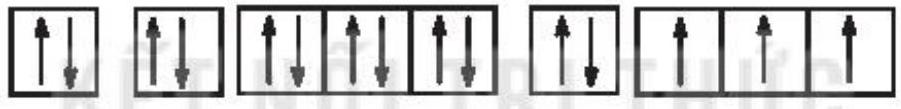
\includegraphics[max width=\textwidth, center]{2025_10_23_ee735750217b2aca435cg-21}\\
c) - Tính chất đơn chất: nguyên tố P là phi kim trung bình:

\begin{itemize}
  \item Phản ứng với oxygen tạo oxide.
  \item Phản ứng với chlorine tạo phosphorus chloride.
  \item Phản ứng với kim loại tạo phosphide.
\end{itemize}

\begin{itemize}
  \item Tính chất hợp chất: $\mathrm{P}_{2} \mathrm{O}_{5}$ là acidic oxide phản ứng với nước tạo hydroxide tương ứng $\mathrm{H}_{3} \mathrm{PO}_{4}$ là acid.\\
9.16. Số $\mathrm{mol} \mathrm{H}_{2}=0,025 \mathrm{~mol}$; số $\mathrm{mol} \mathrm{Na}_{2} \mathrm{SO}_{4}$ là $0,009 \mathrm{~mol}$ và $0,0105 \mathrm{~mol}$.
\end{itemize}

Kí hiệu hai kim loại kiềm kế tiếp là M , có nguyên tử khối trung bình là $\overline{\mathrm{M}}$.

$$
\begin{aligned}
& \mathrm{Ba}+2 \mathrm{H}_{2} \mathrm{O} \rightarrow \mathrm{Ba}(\mathrm{OH})_{2}+\mathrm{H}_{2} \\
& 2 \mathrm{M}+2 \mathrm{H}_{2} \mathrm{O} \rightarrow 2 \mathrm{MOH}+\mathrm{H}_{2}
\end{aligned}
$$

$\mathrm{Ba}(\mathrm{OH})_{2}+\mathrm{Na}_{2} \mathrm{SO}_{4} \rightarrow \mathrm{BaSO}_{4}+2 \mathrm{NaOH}$ ( số $\mathrm{mol} \mathrm{Ba}^{2+}=$ số $\mathrm{mol} \mathrm{SO}_{4}^{2-}$ )\\
Khi thêm $0,009 \mathrm{~mol} \mathrm{Na}_{2} \mathrm{SO}_{4}, \mathrm{Ba}^{2+}$ dư: số $\mathrm{mol} \mathrm{Ba}=$ số $\mathrm{mol} \mathrm{Ba}^{2+}>0,009 \mathrm{~mol}$.

Khi thêm $0,0105 \mathrm{~mol} \mathrm{Na}_{2} \mathrm{SO}_{4}, \mathrm{SO}_{4}^{2-}$ dư: số $\mathrm{mol} \mathrm{Ba}=$ số $\mathrm{mol} \mathrm{Ba}^{2+}<0,0105 \mathrm{~mol}$. Coi số mol Ba và $M$ lần lượt là $x$ và $y$.\\
Ta có: $137 \mathrm{x}+\overline{\mathrm{M}} \mathrm{y}=2,3$\\
và


\begin{equation*}
x+0,5 y=0,025 \tag{I}
\end{equation*}


Với $0,009<\mathrm{x}<0,0105 \Rightarrow 0,019<\mathrm{y}<0,032$.\\
Ghép (I) và (II), ta được: $(68,5-\overline{\mathrm{M}}) \mathrm{y}=1,125$ hay $\mathrm{y}=\frac{1,125}{68,5-\overline{\mathrm{M}}}$\\
$0,019<\frac{1,125}{68,5-\overline{\mathrm{M}}}<0,032 \Rightarrow 26,92<\overline{\mathrm{M}}<36,79$.\\
$\Rightarrow$ Hai kim loại kiềm thoả mãn đề bài là sodium (23) và potassium (39).

\section*{CHUONG 3 LIÊN KẾT HOÁ HỌC}
\begin{table}[h]
\begin{center}
\captionsetup{labelformat=empty}
\caption{Bài 10. QUY TÁC OCTET}
\begin{tabular}{|c|c|c|c|c|c|c|}
\hline
10.1. B & 10.2. D & 10.3. A & 10.4. B & 10.5. C & 10.6. D & 10.7. B \\
\hline
\end{tabular}
\end{center}
\end{table}

10.8. - Nguyên tử khí hiếm đều có cấu hình electron bão hoà là $\mathrm{ns}^{2} \mathrm{np}^{6}$ (trự helium có cấu hình $1 \mathrm{~s}^{2}$ ) làm cho nguyên tử khí hiếm rất bền vững nên các nguyên tử khí hiếm rất khó tham gia phản ứng hoá học. Trong tự nhiên, các khí hiếm đều tồn tại ở trạng thái nguyên tử (hay còn gọi là phân tử một nguyên tử) tự do, bền vững (nên còn gọi là các khí trơ).

\begin{itemize}
  \item Nguyên tử của các nguyên tố khác có xu hướng liên kết với nhau để đạt được cấu hình electron bền vững của khí hiếm, ví dự: $\mathrm{H}_{2}, \mathrm{Cl}_{2}, \mathrm{HCl}, \mathrm{CO}_{2}, \ldots$ hay tự tập hợp lại thành các khối tinh thể, ví dự: tinh thể $\mathrm{NaCl}, \ldots$\\
10.9. - Nguyên tử potassium chỉ có 1 electron ở lớp ngoài cùng nên dễ dàng nhường đi electron này để tạo thành ion dương. Ion dương $\left(\mathrm{K}^{+}\right)$có cấu hình electron lớp ngoài cùng giống với khí hiếm argon ( $3 s^{2} 3 p^{6}$ ) đứng trước potassium trong bảng tuần hoàn.
  \item Nguyên tử bromine có 7 electron ở lớp electron ngoài cùng nên dễ dàng nhận thêm 1 electron tạo ra anion bromide ( $\mathrm{Br}^{-}$) có cấu hình electron lớp ngoài cùng giống với khí hiếm krypton ( $4 \mathrm{~s}^{2} 4 \mathrm{p}^{6}$ ), đứng sau bromine trong bảng tuần hoàn.\\
10.10. - Khi hình thành liên kết $\mathrm{H}+\mathrm{Cl} \rightarrow \mathrm{H}-\mathrm{Cl}$ thì hệ toả ra năng lượng và ngược lại khi phá vỡ liên kết $\mathrm{H}-\mathrm{Cl} \rightarrow \mathrm{H}+\mathrm{Cl}$ thì hệ thu thêm năng lượng.
  \item Xét về mặt năng lượng thì phân tử $\mathrm{H}-\mathrm{Cl}$ có năng lượng nhỏ hơn hệ hai nguyên tử H và Cl riêng rẽ. Trong hai hệ đó thì hệ $\mathrm{H}-\mathrm{Cl}$ bền hơn hệ H và Cl .\\
10.11. Cấu hình electron của nguyên tử Na :\\
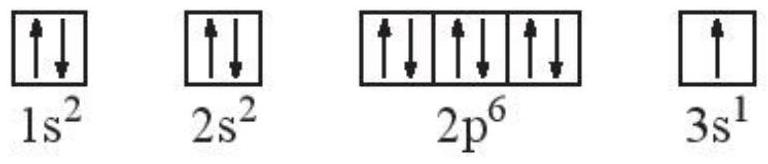
\includegraphics[max width=\textwidth, center]{2025_10_23_ee735750217b2aca435cg-23(1)}
\end{itemize}

Cấu hình electron của nguyên tử S :\\
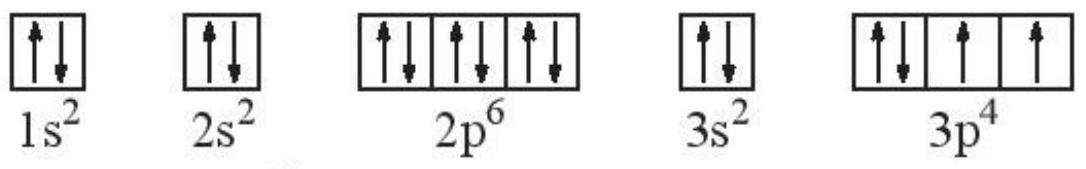
\includegraphics[max width=\textwidth, center]{2025_10_23_ee735750217b2aca435cg-23}

Khi Na kết hợp với S , mỗi nguyên tử Na nhường đi 1 electron hoá trị duy nhất để tạo thành cation $\mathrm{Na}^{+}$có 8 electron ở vỏ nguyên tử giống với khí hiếm neon. Nguyên tử S có 6 electron hoá trị nhận thêm 2 electron từ hai nguyên tử Na tạo thành ion sulfide $\mathrm{S}^{2-}$ có 8 electron ở vỏ nguyên tử giống với khí hiếm argon.

Hai nguyên tử Na và S đều đạt cấu hình electron bão hoà theo quy tắc octet trong phân tử sodium sulfide $\mathrm{Na}_{2} \mathrm{~S}$.\\
10.12. - Phân tử $\mathrm{O}_{2}$ :

$$
: \ddot{o}:+: \ddot{o}: \longrightarrow: \ddot{o}:: \ddot{o}: \text { hay }: \ddot{o}=\ddot{o}:
$$

\begin{itemize}
  \item Phân tử $\mathrm{CO}_{2}$ :
\end{itemize}

$$
: \ddot{\mathrm{O}}:+: c:+: \ddot{\mathrm{O}}: \longrightarrow \text { :o }:: c:: \circ \cdot \text { hay }: \dot{\mathrm{O}}=c=0:
$$

\begin{itemize}
  \item Phân tử KBr:
\end{itemize}

$$
\mathrm{K} \cdot+: \ddot{\mathrm{Br}} \cdot \longrightarrow[\mathrm{~K}]^{+}+[: \ddot{\mathrm{Br}}:]^{-}
$$

\begin{itemize}
  \item Phân tử $\mathrm{CaCl}_{2}$ :\\
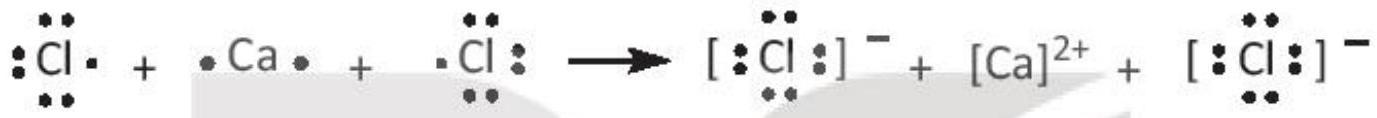
\includegraphics[max width=\textwidth, center]{2025_10_23_ee735750217b2aca435cg-24(1)}\\
10.13. $-\mathrm{CaCO}_{3}$ :\\
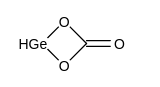
\includegraphics{smile-175b6c8036196aed62008b980eed9df51d3246d7}\\
$-\mathrm{Ba}\left(\mathrm{NO}_{3}\right)_{2}$ :\\
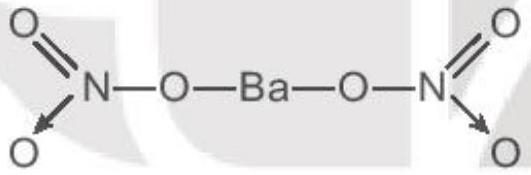
\includegraphics[max width=\textwidth, center]{2025_10_23_ee735750217b2aca435cg-24}\\
$-\mathrm{Al}_{2}\left(\mathrm{SO}_{4}\right)_{3}:$\\
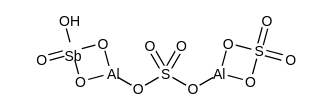
\includegraphics{smile-8ea47c5ac04851accf586b0e33dd3d54a4e29bb1}\\
10.14. a) A thuộc nhóm IVA và $D$ thuộc nhóm VIA $\Rightarrow$ số oxi hoá cao nhất của A trong X là +4 còn số oxi hoá của D trong X là -2 .\\
Công thức phân tử X có dạng $\mathrm{AD}_{2}$. Ta có: $\mathrm{A}+2 \mathrm{D}=76$.\\
$\Rightarrow$ Nguyên tử khối trung bình của $A, D$ là: $\frac{76}{3}=25,33$.\\
$\Rightarrow A$ và $D$ thuộc chu kì $2,3 \Rightarrow$ Có các cặp nguyên tố sau:\\
$\mathrm{C}=12$ và $\mathrm{O}=16 ; \mathrm{C}=12$ và $\mathrm{S}=32 ; \mathrm{Si}=28$ và $\mathrm{O}=16 ; \mathrm{Si}=28$ và $\mathrm{S}=32$.\\
$\mathrm{C}=12$ và $\mathrm{S}=32$ thoả mãn $\mathrm{A}+2 \mathrm{D}=76 \Rightarrow$ Công thức $\mathrm{X}: \mathrm{CS}_{2}$.\\
b) Đề xuất công thức cấu tạo: $\stackrel{\circ}{\circ} \mathrm{S}=\mathrm{C}=\mathrm{S}_{\circ}^{\circ} . \mathrm{CS}_{2}$ có cấu trúc thẳng giống $\mathrm{CO}_{2}$.
\end{itemize}

Các nguyên tử $C$ và $S$ đều có 8 electron lớp ngoài cùng theo quy tắc octet.

\section*{Bài 11. LIÊN KẾT ION}
\begin{center}
\begin{tabular}{|l|l|l|l|}
\hline
$11.1 . \mathrm{C}$ & $11.2 . \mathrm{A}$ & $11.3 . \mathrm{D}$ & $11.4 . \mathrm{B}$ \\
\hline
$11.5 . \mathrm{C}$ & $11.6 . \mathrm{B}$ & $11.7 . \mathrm{B}$ & $11.8 . \mathrm{C}$ \\
\hline
\end{tabular}
\end{center}

11.9. Phương trình biểu diễn sự hình thành các ion:\\
$\mathrm{K} \rightarrow \mathrm{K}^{+}+1 \mathrm{e}$\\
$\mathrm{Be} \rightarrow \mathrm{Be}^{2+}+2 \mathrm{e}$\\
$\mathrm{Cr} \rightarrow \mathrm{Cr}^{3+}+3 \mathrm{e}$\\
$\mathrm{F}+\mathrm{e} \rightarrow \mathrm{F}^{-}$\\
$\mathrm{Se}+2 \mathrm{e} \rightarrow \mathrm{Se}^{2-}$\\
$\mathrm{N}+3 \mathrm{e} \rightarrow \mathrm{N}^{3-}$\\
11.10. a) Cấu hình electron:

\[
\begin{array}{lll}
20 \mathrm{Ca}^{2+}: 1 \mathrm{~s}^{2} 2 \mathrm{~s}^{2} 2 \mathrm{p}^{6} 3 \mathrm{~s}^{2} 3 \mathrm{p}^{6} & \text { (I) } 13 \mathrm{Al}^{3+}: 1 \mathrm{~s}^{2} 2 \mathrm{~s}^{2} 2 \mathrm{p}^{6} \\
9 \mathrm{~F}^{-}: 1 \mathrm{~s}^{2} 2 \mathrm{~s}^{2} 2 \mathrm{p}^{6} & \text { (III) } 16 \mathrm{~S}^{2-}: 1 \mathrm{~s}^{2} 2 \mathrm{~s}^{2} 2 \mathrm{p}^{6} 3 \mathrm{~s}^{2} 3 \mathrm{p}^{6} \\
7 \mathrm{~N}^{3-}: 1 \mathrm{~s}^{2} 2 \mathrm{~s}^{2} 2 \mathrm{p}^{6} & \text { (V) } \tag{IV}
\end{array}
\]

b) Các cấu hình (II), (III), (V) giống cấu hình electron của khí hiếm 10 Ne .

Các cấu hình (I), (IV) giống cấu hình electron của khí hiếm 18 Ar .\\
11.11. Các hợp chất ion thường là chất rắn ở nhiệt độ phòng vì hợp chất ion có cấu trúc mạng tinh thể ion. Lực tĩnh điện mạnh giữa các phần tử mạng với nhau làm cho khoảng cách giữa các phần tử ngắn lại.\\
11.12. Những phân tử có liên kết ion là: $\mathrm{K}_{2} \mathrm{O}, \mathrm{K}_{2} \mathrm{~S}, \mathrm{NaCl}, \mathrm{CaF}_{2}$.\\
11.13. Các hợp chất ion là: $\mathrm{KF}, \mathrm{K}_{2} \mathrm{O}, \mathrm{CaF}_{2}, \mathrm{CaO}$.\\
11.14. a) Magnesium fluoride:

$$
: \ddot{\mathrm{F}} .+\mathrm{Mg}:+\cdot \ddot{\mathrm{F}}: \rightarrow[: \ddot{\mathrm{F}}:]^{-}+[\mathrm{Mg}]^{2+}+[: \ddot{\mathrm{F}}:]^{-} \rightarrow \mathrm{MgF}_{2}
$$

b) Potassium fluoride:

$$
K \cdot+: \ddot{F}: \rightarrow[K]^{+}+[: \ddot{F}:]^{-} \rightarrow K F
$$

c) Sodium oxide:

$$
\mathrm{Na} \cdot+\ddot{0 .}{ }_{0 .}+\cdot \mathrm{Na} \rightarrow[\mathrm{Na}]^{+}+[: \ddot{0 .}:]^{2-}+\left[\mathrm{Na}^{+} \rightarrow \mathrm{Na}_{2} \mathrm{O}\right.
$$

d) Calcium oxide:

$$
\cdot \mathrm{Ca} \cdot+\cdot \ddot{0} \cdot \rightarrow[\mathrm{Ca}]^{2+}+[: \underset{: O}{: O}:]^{2-} \rightarrow \mathrm{CaO}
$$

11.15. a) Khi nhận electron, nguyên tử X biến thành anion $\mathrm{X}^{-}$.

Cấu hình electron của $X$ là $1 s^{2} 2 s^{2} 2 p^{6} 3 s^{2} 3 p^{5}, X$ là chlorine.\\
X là phi kim điển hình.\\
b) Barium là nguyên tố kim loại điển hình ở chu kì 6 , nhóm IIA. Barium dễ nhường 2 electron hoá trị và tạo ra cation có điện tích $2+$. Khi chlorine kết hợp với barium, nguyên tử barium nhường 2 electron cho hai nguyên tử chlorine (mỗi nguyên tử chlorine nhận 1 electron), tạo thành các ion $\mathrm{Ba}^{2+}$ và $\mathrm{Cl}^{-}$. Các ion này mang điện trái dấu sẽ hút nhau tạo thành liên kết ion.\\
11.16. a) Nguyên tử $X$ chỉ có 7 electron trên phân lớp $s$ nên cấu hình electron của $X$ là: $1 s^{2} 2 s^{2} 2 p^{6} 3 s^{2} 3 p^{6} 4 s^{1}$.\\
Nguyên tử $Z$ chỉ có 17 e trên phân lớp $p$ nên cấu hình electron của $Z$ là:

$$
1 s^{2} 2 s^{2} 2 p^{6} 3 s^{2} 3 p^{6} 4 s^{2} 3 d^{10} 4 p^{5} .
$$

$\Rightarrow \mathrm{X}$ là ${ }_{19} \mathrm{~K}$ và Z là ${ }_{35} \mathrm{Br}$.\\
$\Rightarrow$ Công thức hoá học của hợp chất tạo bởi X và Z là KBr .\\
b) Hợp chất KBr có tính dẫn điện khi nóng chảy hoặc tan trong dung dịch vì nó là hợp chất ion.\\
c) Trong thực tế, KBr được sử dụng rộng rãi như thuốc chống co giật và an thần, nó là muối ion điển hình, hoàn toàn phân cực và đạt độ $\mathrm{pH}=7$ trong dung dịch nước.

\section*{Bài 12. LIÊN KẾT CỘNG HOÁ TR!}
\begin{center}
\begin{tabular}{|l|l|l|l|l|l|}
\hline
$12.1 . \mathrm{D}$ & $12.2 . \mathrm{D}$ & $12.3 . \mathrm{B}$ & $12.4 . \mathrm{D}$ & $12.5 . \mathrm{A}$ & $12.6 . \mathrm{B}$ \\
\hline
$12.7 . \mathrm{A}$ & $12.8 . \mathrm{C}$ & $12.9 . \mathrm{C}$ & $12.10 . \mathrm{D}$ & $12.11 . \mathrm{C}$ & $12.12 . \mathrm{D}$ \\
\hline
\end{tabular}
\end{center}

12.13. Tuy có độ âm điện của chlorine và nitrogen gần bằng nhau nhưng do trong phân tử $\mathrm{Cl}_{2}$ có liên kết đơn $\sigma(\mathrm{Cl}-\mathrm{Cl})$ còn trong phân tử $\mathrm{N}_{2}$ có liên kết ba $(\mathrm{N} \equiv \mathrm{N})$ gồm 1 liên kết $\sigma$ và 2 liên kết $\pi$ rất bền vững. Năng lượng cần để phá vỡ liên kết ba trong phân tử $\mathrm{N}_{2}$ lớn hơn nhiều so với năng lượng cần để phá vỡ một liên kết đơn trong phân tử $\mathrm{Cl}_{2}$. Do đó, ở điều kiện thường, $\mathrm{N}_{2}$ hoạt động kém $\mathrm{Cl}_{2}$.\\
12.14. a) Công thức Lewis của các phân tử:

\begin{center}
\begin{tabular}{|c|c|c|c|}
\hline
$\mathrm{F}_{2}$ & $\mathrm{~N}_{2}$ & $\mathrm{CO}_{2}$ & $\mathrm{H}_{2} \mathrm{O}$ \\
\hline
$\ddot{\mathrm{F}}-\ddot{\mathrm{F}}:$ & $: \mathrm{N} \equiv \mathrm{N}:$ & $: \stackrel{\circ}{\mathrm{O}}=\mathrm{C}=\mathrm{O}^{\cdot} \cdot$ & $\mathrm{H}-\ddot{\mathrm{O}}-\mathrm{H}$ \\
\hline
\end{tabular}
\end{center}

b) Phân tử chứa liên kết cộng hoá trị không phân cực: $\mathrm{N}_{2}, \mathrm{~F}_{2}$.

Phân tử chứa liên kết cộng hoá trị phân cực: $\mathrm{H}_{2} \mathrm{O}, \mathrm{CO}_{2}$.\\
Phân tử phân cực: $\mathrm{H}_{2} \mathrm{O}$.\\
Phân tử không phân cực: $\mathrm{N}_{2}, \mathrm{~F}_{2}, \mathrm{CO}_{2}$.\\
12.15. a) Phân tử có liên kết cộng hoá trị không phân cực: $\mathrm{Br}_{2}$.

Phân tử có liên kết cộng hoá trị phân cực: $\mathrm{H}_{2} \mathrm{~S}, \mathrm{CH}_{4}, \mathrm{NH}_{3}, \mathrm{C}_{2} \mathrm{H}_{4}$ và $\mathrm{C}_{2} \mathrm{H}_{2}$.\\
b) Phân tử chỉ có liên kết đơn: $\mathrm{H}_{2} \mathrm{~S}, \mathrm{CH}_{4}, \mathrm{NH}_{3}$ và $\mathrm{Br}_{2}$.

Phân tử có liên kết đôi: $\mathrm{CH}_{2}=\mathrm{CH}_{2}$.\\
Phân tử có liên kết ba: $\mathrm{CH} \equiv \mathrm{CH}$.\\
12.16. a) - 3); b) - 4); c) - 2); d) - 1).

Nước, băng phiến, butane là các hợp chất cộng hoá trị, phân tử có độ phân cực không cao nên dễ tách ra khỏi nhau khi đun nóng. Ngược lại, NaCl là tinh thể ion có lực hút mạnh giữa các ion nên khó tách ra khỏi nhau và nhiệt độ nóng chảy cao.

\section*{Bài 13. LIÊN KẾT HYDROGEN VÀ TƯƠNG TÁC VAN DER WAALS}
\begin{center}
\begin{tabular}{|l|l|l|l|l|l|}
\hline
$13.1 . \mathrm{D}$ & $13.2 . \mathrm{C}$ & $13.3 . \mathrm{C}$ & $13.4 . \mathrm{B}$ & $13.5 . \mathrm{D}$ & $13.6 . \mathrm{A}$ \\
\hline
$13.7 . \mathrm{D}$ & $13.8 . \mathrm{D}$ & $13.9 . \mathrm{C}$ & $13.10 . \mathrm{B}$ & $13.11 . \mathrm{C}$ & $13.12 . \mathrm{C}$ \\
\hline
\end{tabular}
\end{center}

13.13. $\mathrm{CH}_{3} \mathrm{OH}$ và $\mathrm{CH}_{3} \mathrm{COOH}$ chứa nguyên tử O có độ âm điện lớn $(3,44)$ và nguyên tử H liên kết với nguyên tử O trong nhóm -OH là nguyên tử hydrogen linh động tạo ra liên kết hydrogen:

$$
\cdots \mathrm{O}-\mathrm{H} \cdots \mathrm{O}-\mathrm{H} \cdots
$$

13.14. Nhiệt độ sôi của $\mathrm{H}_{2} \mathrm{O}$ lớn hơn rất nhiều so với $\mathrm{NH}_{3}$ và $\mathrm{CH}_{4}$ vì phân tử $\mathrm{H}_{2} \mathrm{O}$ và $\mathrm{NH}_{3}$ có liên kết hydrogen liên phân tử (còn $\mathrm{CH}_{4}$ không có); do độ âm điện $\mathrm{O}>\mathrm{N}$ nên liên kết hydrogen trong $\mathrm{H}_{2} \mathrm{O}$ bền hơn trong $\mathrm{NH}_{3}$.\\
13.15. Dung dịch ethanol có $\mathrm{C}_{2} \mathrm{H}_{5} \mathrm{OH}$ và $\mathrm{H}_{2} \mathrm{O}$, cả hai phân tử này đều chứa nguyên tử O có độ âm điện lớn $(3,44)$ và nguyên tử H liên kết với nguyên tử O trong nhóm -OH là nguyên tử hydrogen linh động tạo ra liên kết hydrogen.\\
Có bốn kiểu liên kết hydrogen trong dung dịch ethanol: alcohol - alcohol; nước - nước; alcohol - nước và nước - alcohol.\\
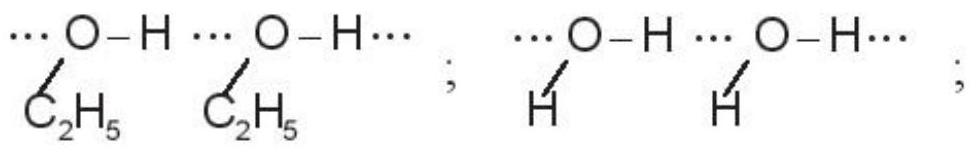
\includegraphics[max width=\textwidth, center]{2025_10_23_ee735750217b2aca435cg-28}\\
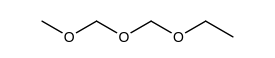
\includegraphics{smile-c1976842053c97f21ba23c5514c7c9ee39bcbcee}

Liên kết hydrogen càng bền khi nguyên tử có độ âm điện lớn hơn và nguyên tử H linh động hơn. Trong bốn kiểu trên: kiểu bền nhất là liên kết giữa H của nước với O của alcohol (nước - alcohol). Kiểu kém bền nhất là liên kết giữa H của alcohol với O của alcohol (alcohol - alcohol).\\
13.16. - Số liên kết hydrogen trung bình được tạo thành trên mỗi phân tử phụ thuộc vào:

\begin{itemize}
  \item Số nguyên tử hydrogen liên kết với $\mathrm{F}, \mathrm{O}$ hoặc N trong phân tử.
  \item Số lượng các cặp electron chưa liên kết có mặt trên $\mathrm{F}, \mathrm{O}, \mathrm{N}$.
\end{itemize}

\begin{itemize}
  \item Mỗi phân tử nước có hai nguyên tử hydrogen và hai cặp electron chưa liên kết nên phân tử nước có nhiều liên kết hydrogen với các phân tử nước khác. Nó có mức trung bình là hai liên kết hydrogen trên mỗi phân tử.
  \item Ammonia có it liên kết hydrogen hơn nước. Trung bình nó có thể hình thành chỉ một liên kết hydrogen trên mỗi phân tử. Mặc dù mỗi phân tử ammonia có ba nguyên tử hydrogen gắn với nguyên tử nitrogen, nhưng nó chỉ có một cặp electron duy nhất có thể tham gia vào quá trình hình thành liên kết hydrogen.\\
13.17. Khi chưng cất dầu mỏ, butane sẽ bay hơi trước octane. Vì octane $(M=114)$ có phân tử khối lớn hơn butane $(M=58)$ nên có nhiệt độ sôi cao hơn.\\
13.18. - Giá trị nhiệt độ sôi của từng chất:
\end{itemize}

$$
\mathrm{H}_{2} \mathrm{O}\left(100^{\circ} \mathrm{C}\right) ; \mathrm{H}_{2} \mathrm{~S}\left(-61^{\circ} \mathrm{C}\right) ; \mathrm{H}_{2} \mathrm{Se}\left(-42^{\circ} \mathrm{C}\right) \text { và } \mathrm{H}_{2} \mathrm{Te}\left(-2^{\circ} \mathrm{C}\right) .
$$

\begin{itemize}
  \item Giải thích: sự tăng nhiệt độ sôi từ $\mathrm{H}_{2} \mathrm{~S}$ đến $\mathrm{H}_{2} \mathrm{Te}$ là do khối lượng phân tử tăng lên. Nếu $\mathrm{H}_{2} \mathrm{O}$ chỉ có lực van der Waals giữa các phân tử thì nhiệt độ sôi của nó dự đoán vào khoảng $-80^{\circ} \mathrm{C}$. Tuy nhiên, nhiệt độ sôi của $\mathrm{H}_{2} \mathrm{O}$ là $100^{\circ} \mathrm{C}$, cao hơn nhiều, đó là vì phân tử $\mathrm{H}_{2} \mathrm{O}$ còn có liên kết hydrogen liên phân tử, làm cho liên kết giữa các phân tử $\mathrm{H}_{2} \mathrm{O}$ bền vững hơn.
\end{itemize}

\begin{table}[h]
\begin{center}
\captionsetup{labelformat=empty}
\caption{Bài 14. ÔN TẬP CHUƠNG 3}
\begin{tabular}{|l|l|l|l|l|}
\hline
14.1. B & $14.2 . \mathrm{D}$ & $14.3 . \mathrm{D}$ & $14.4 . \mathrm{C}$ & $14.5 . \mathrm{D}$ \\
\hline
$14.6 . \mathrm{A}$ & $14.7 . \mathrm{A}$ & $14.8 . \mathrm{C}$ & $14.9 . \mathrm{A}$ & $14.10 . \mathrm{B}$ \\
\hline
\end{tabular}
\end{center}
\end{table}

14.11. Nguyên tử trung tâm $S$ có 6 electron lớp ngoài cùng và nguyên tử $O$ cũng có 6 electron lớp ngoài cùng. Khi tạo thành phân tử $\mathrm{SO}_{3}$, nguyên tử S và 1 nguyên tử O dùng chung 2 cặp electron để tạo 2 liên kết cộng hoá trị kép phân cực. Để thoả mãn quy tắc octet, liên kết cộng hoá trị giữa nguyên tử S và 2 nguyên tử O còn lại được thực hiện bằng sự cho - nhận 2 cặp electron của nguyên tử S . Kết quả, trong phân tử $\mathrm{SO}_{3}$, các nguyên tử S và O đều có 8 electron lớp ngoài cùng thoã mãn quy tắc octet.\\
Công thức Lewis:\\
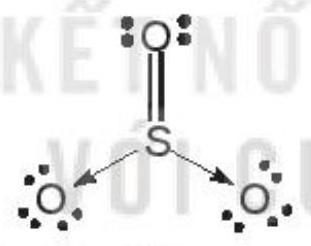
\includegraphics[max width=\textwidth, center]{2025_10_23_ee735750217b2aca435cg-29}\\
14.12. Sự hình thành các liên kết trong phân tử NaClO :

Nguyên tử Na có 1 electron lớp ngoài cùng, nguyên tử $O$ có 6 electron lớp ngoài cùng và nguyên tử Cl có 7 electron lớp ngoài cùng.\\
Nguyên tử Na nhường đi 1 electron để trở thành ion $\mathrm{Na}^{+}$, có cấu hình electron bền vững của khí hiếm Ne . Nhóm nguyên tử OCl nhận thêm 1 electron để trở thành ion $\mathrm{OCl}^{-}$. Các ion này mang điện trái dấu sẽ hút nhau tạo thành liên kết ion.\\
Ion $\mathrm{OCl}^{-}$có 14 electron hoá trị:\\
6 (đối với O$)+7$ (đối với Cl ) +1 (đối với điện tích âm) $=14$ hay 7 cặp electron hoá trị. Sau khi tạo thành liên kết $\mathrm{O}-\mathrm{Cl}$ và phân bố 6 cặp electron còn lại chưa liên kết vào các nguyên tử, cả hai nguyên tử đều có 8 electron lớp ngoài cùng.

Công thức Lewis: $\mathrm{Na}^{+}$\\
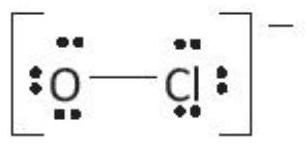
\includegraphics[max width=\textwidth, center]{2025_10_23_ee735750217b2aca435cg-30}\\
14.13. a) $\mathrm{C}_{2} \mathrm{H}_{4}$ có 5 liên kết $\sigma$ và 1 liên kết $\pi$.\\
b) $\mathrm{C}_{2} \mathrm{H}_{2}$ có 3 liên kết $\sigma$ và 2 liên kết $\pi$.\\
c) HCN có 2 liên kết $\sigma$ và 2 liên kết $\pi$.\\
d) HCOOH có 4 liên kết $\sigma$ và 1 liên kết $\pi$.\\
14.14. Bản chất các liên kết phụ thuộc vào hiệu độ âm điện giữa hai nguyên tử của hai nguyên tố tạo liên kết. Viết công thức cấu tạo các phân tử và tính hiệu độ âm điện để suy ra bản chất liên kết.

\begin{itemize}
  \item $\mathrm{H}-\mathrm{Cl}=\mathrm{O}$ có hiệu độ âm điện $\mathrm{H}-\mathrm{Cl}$ là $0,96 \Rightarrow$ liên kết cộng hoá trị phân cực; $\mathrm{Cl}-\mathrm{O}$ là $0,28 \Rightarrow$ liên kết cộng hoá trị không phân cực.
  \item $\mathrm{K}^{+}$và $[\mathrm{S}-\mathrm{H}]^{-}$có hiệu độ âm điện K và S là $1,76 \Rightarrow$ liên kết ion; $\mathrm{S}-\mathrm{H}$ là $0,38 \Rightarrow$ liên kết cộng hoá trị phân cực.\\
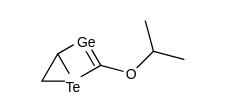
\includegraphics{smile-6a38256abe366e5ecea4b3692930725576666a9c}\\
có hiệu độ âm điện H và O là $1,24 \Rightarrow$ liên kết cộng hoá trị phân cực; $\mathrm{C}-\mathrm{O}$ có hiệu độ âm điện là $0,89 \Rightarrow$ liên kết cộng hoá trị phân cực.\\
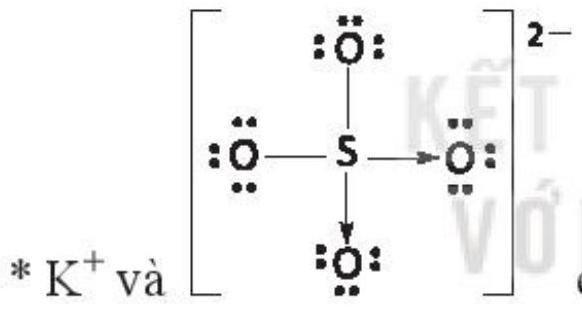
\includegraphics[max width=\textwidth, center]{2025_10_23_ee735750217b2aca435cg-30(1)}\\
có hiệu độ âm điện $\mathrm{K}-\mathrm{O}$ là $2,62 \Rightarrow$ liên kết ion; $\mathrm{S}-\mathrm{O}$ là $1,54 \Rightarrow$ liên kết cộng hoá trị phân cực.\\
14.15. a) Sự tăng nhiệt độ sôi từ HCl đến HI do khối lượng phân tử tăng.\\
b) HF có liên kết hydrogen làm cho các phân tử liên kết với nhau chặt chẽ hơn nên nhiệt độ sôi cao hơn.\\
14.16. a) Coi $x$ và $y$ là số proton (số electron) ở nguyên tử $A$ và $B$ tương ứng.
\end{itemize}

Ta có : $\mathrm{x}+3 \mathrm{y}=42-2=40 \Rightarrow \mathrm{y}<\frac{40}{3}=13,33$.\\
$B$ thuộc chu kì 2 và là một phi kim (tạo anion) nên $B$ chỉ có thể là $F, O$ hoặc $N$.

\begin{itemize}
  \item Nếu B là F thì $\mathrm{y}=9$, trong $\mathrm{AF}_{3}^{2-}$ có A với số oxi hoá bằng +1\\
$\Rightarrow \mathrm{x}=40-(3 \cdot 9)=13 \sim \mathrm{Al}$ (không hợp lí vì Al không có số oxi hoá bằng +1 ).
  \item Khi B là O thì $\mathrm{y}=8$, trong $\mathrm{AO}_{3}^{2-}$ có A với số oxi hoá bằng +4\\
$\Rightarrow \mathrm{x}=40-(3 \cdot 8)=16 \sim \mathrm{~S}$ (lưu huỳnh) $\Rightarrow$ Anion là $\mathrm{SO}_{3}^{2-}$.
  \item Khi B là N thì $\mathrm{y}=7$, trong $\mathrm{AN}_{3}^{2-}$ có A với số oxi hoá bằng +7\\
$\Rightarrow \mathrm{x}=40-(3 \cdot 7)=19 \sim \mathrm{~K}$ (không hợp lí vì K không có số oxi hoá bằng +7 ).\\
b) Cấu tạo Lewis:\\
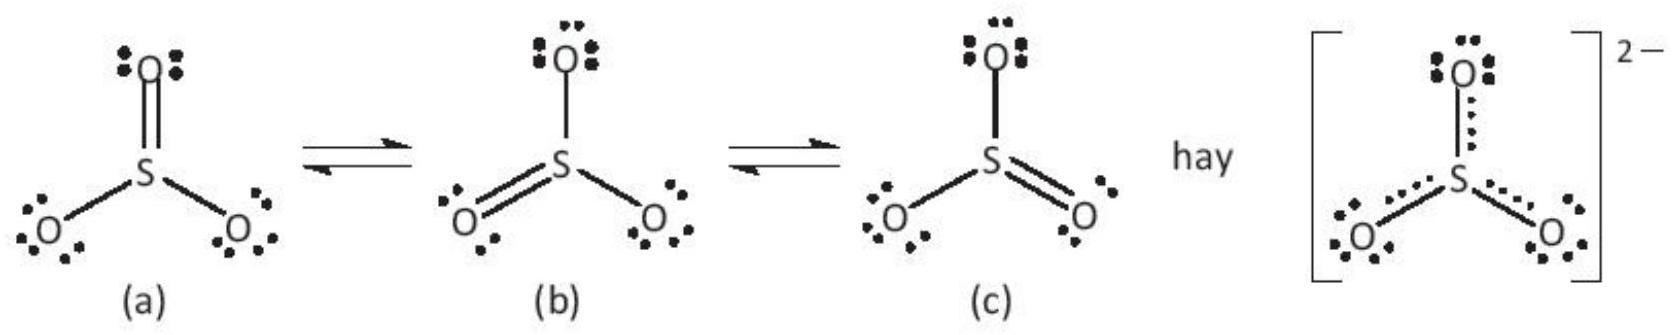
\includegraphics[max width=\textwidth, center]{2025_10_23_ee735750217b2aca435cg-31(1)}\\
14.17. a) Nguyên tố $s$ có 7 electron $s$ là $K\left(1 s^{2} 2 s^{2} \ldots 3 s^{2} \ldots 4 s^{1}\right)$; nguyên tố p có 11 electron p là $\mathrm{Cl}\left(\ldots 2 \mathrm{p}^{6} \ldots 3 \mathrm{p}^{5}\right)$; nguyên tố p có 4 electron p là $\mathrm{O}\left(\ldots 2 \mathrm{p}^{4}\right)$;\\
Khối lượng O trong X là: $122,5 \cdot 0,3919 \approx 48(\mathrm{amu})$ ứng với 3 nguyên tử O .\\
Công thức X có dạng $\mathrm{K}_{\mathrm{x}} \mathrm{Cl}_{\mathrm{y}} \mathrm{O}_{3}$.\\
Theo bài ra ta có: $39 \mathrm{x}+35,5 \mathrm{y}=122,5-48=74,5$.\\
$\Rightarrow \mathrm{x}=\mathrm{y}=1 \Rightarrow$ công thức $\mathrm{X}: \mathrm{KClO}_{3}$.\\
b) Cấu tạo $X$ :\\
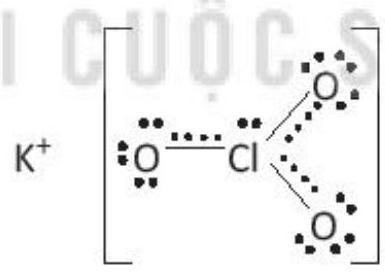
\includegraphics[max width=\textwidth, center]{2025_10_23_ee735750217b2aca435cg-31}\\
gồm liên kết $\mathrm{K}^{+}$và $\mathrm{ClO}_{3}^{-}$là liên kết ion; liên kết đơn $\mathrm{Cl}-\mathrm{O}$ và liên kết kép $\mathrm{Cl}=\mathrm{O}$ là các liên kết cộng hoá trị phân cực.
\end{itemize}

\begin{table}[h]
\begin{center}
\captionsetup{labelformat=empty}
\caption{Bài 15. PHẢN ỨNG OXI HOÁ - KHỦ}
\begin{tabular}{|l|l|l|l|l|l|}
\hline
$15.1 . \mathrm{B}$ & $15.2 . \mathrm{D}$ & $15.3 . \mathrm{A}$ & $15.4 . \mathrm{D}$ & $15.5 . \mathrm{C}$ & $15.6 . \mathrm{A}$ \\
\hline
$15.7 . \mathrm{B}$ & $15.8 . \mathrm{B}$ & $15.9 . \mathrm{C}$ & $15.10 . \mathrm{A}$ & $15.11 . \mathrm{B}$ & $15.12 . \mathrm{C}$ \\
\hline
$15.13 . \mathrm{D}$ & $15.14 . \mathrm{D}$ & $15.15 . \mathrm{B}$ & $15.16 . \mathrm{C}$ & $15.17 . \mathrm{D}$ & $15.18 . \mathrm{C}$ \\
\hline
\end{tabular}
\end{center}
\end{table}

15.19. a) $\quad \stackrel{-4}{\mathrm{C}} \mathrm{H}_{4}+\stackrel{-2}{\mathrm{O}}{ }_{2} \xrightarrow{\mathrm{t}^{\circ}} \stackrel{+4}{\mathrm{C}} \mathrm{O}_{2}+\mathrm{H}_{2} \mathrm{O}^{-2}$

$$
\begin{aligned}
& \stackrel{-4}{\mathrm{C}} \longrightarrow \stackrel{+4}{\mathrm{C}}+8 \mathrm{e}: \text { quá trình oxi hoá } \\
& \stackrel{0}{\mathrm{O}}_{2}+4 \mathrm{e} \longrightarrow 2 \mathrm{O}^{-2}: \text { quá trình khử }
\end{aligned}
$$

b) Lập phương trình hoá học của phản ứng theo phương pháp thăng bằng electron:

$$
\begin{aligned}
& 1 \times \left\lvert\, \begin{array}{l}
-4 \\
\mathrm{C} \\
0 \\
\mathrm{O}_{2}+4 \mathrm{e} \longrightarrow \mathrm{C}^{-2} \mathrm{O}
\end{array}\right.
\end{aligned}
$$

Xác định được hệ số của $\mathrm{CH}_{4}$ và $\mathrm{CO}_{2}$ đều là 1 , hệ số của $\mathrm{O}_{2}$ là 2 , sau đó cân bằng nguyên tố H tìm được hệ số của $\mathrm{H}_{2} \mathrm{O}$ là 2 :

$$
\mathrm{CH}_{4}+2 \mathrm{O}_{2} \xrightarrow{\mathrm{t}^{\circ}} \mathrm{CO}_{2}+2 \mathrm{H}_{2} \mathrm{O} \text {. }
$$

15.20. a) $\quad \stackrel{\mathrm{Na}}{\mathrm{Na}} \stackrel{-1}{\mathrm{Cl}}+\stackrel{+1}{\mathrm{H}_{2}} \mathrm{O} \xrightarrow[\text { max }]{\text { dpdd }} \mathrm{NaOH}+\stackrel{0}{\mathrm{Cl}_{2}}+\stackrel{0}{\mathrm{H}_{2}}$\\
$2 \mathrm{Cl}^{-1} \longrightarrow \mathrm{Cl}_{2}^{0}+2 \mathrm{e}: \mathrm{NaCl}$ là chất khử\\
$2 \stackrel{+1}{\mathrm{H}}+2 \mathrm{e} \longrightarrow \stackrel{0}{\mathrm{H}}_{2}: \mathrm{H}_{2} \mathrm{O}$ là chất oxi hoá\\
b) Lập phương trình hoá học của phản ứng theo phương pháp thăng bằng electron:

$$
\begin{aligned}
& 1 \times \left\lvert\, \begin{array}{ll}
-1 & 0 \\
2 \mathrm{Cl} & \mathrm{Cl}_{2}+2 \mathrm{e} \\
+1 & 0 \\
2 \mathrm{H}+2 \mathrm{e} & \mathrm{H}_{2}
\end{array}\right.
\end{aligned}
$$

Xác định được hệ số của NaCl và NaOH đều là 2 , hệ số của $\mathrm{Cl}_{2}$ và $\mathrm{H}_{2}$ đều là 1 , sau đó cân bằng nguyên tố H tìm được hệ số của $\mathrm{H}_{2} \mathrm{O}$ là 2 :

$$
2 \mathrm{NaCl}+2 \mathrm{H}_{2} \mathrm{O} \xrightarrow[\operatorname{mnx}]{\text { dpdd }} 2 \mathrm{NaOH}+\mathrm{Cl}_{2}+\mathrm{H}_{2} \text {. }
$$

15.21. a) $\mathrm{Zn} \stackrel{-2}{\mathrm{~S}}^{+}+\stackrel{0}{\mathrm{O}}_{2} \xrightarrow{\mathrm{t}^{\circ}} \mathrm{Zn} \stackrel{-2}{\mathrm{O}}^{+}+\stackrel{+4}{\mathrm{~S}^{\circ}} \mathrm{O}_{2}$

$$
\begin{aligned}
& \stackrel{-2}{\mathrm{~S}} \longrightarrow \stackrel{+4}{\mathrm{~S}}+6 \mathrm{e}: \text { quá trình oxi hoá } \\
& \stackrel{0}{\mathrm{O}}_{2}+4 \mathrm{e} \xrightarrow{\mathrm{t}^{\circ}} 2 \mathrm{O}^{-2}: \text { quá trình khử }
\end{aligned}
$$

b) Lập phương trình hoá học của phản ứng theo phương pháp thăng bằng electron:

$$
2 \times\left.\right|^{-2} \stackrel{\text { S }}{0} \longrightarrow \stackrel{+4}{\mathrm{~S}}+6 \mathrm{e}
$$

Xác định được hệ số của $\mathrm{ZnS}, \mathrm{ZnO}$ và $\mathrm{SO}_{2}$ đều là 2 , hệ số của $\mathrm{O}_{2}$ là 3 :

$$
2 \mathrm{ZnS}+3 \mathrm{O}_{2} \xrightarrow{\mathrm{t}^{\circ}} 2 \mathrm{ZnO}+2 \mathrm{SO}_{2}
$$

15.22. a) $\stackrel{-2,5}{\mathrm{C}_{4}} \mathrm{H}_{10}+\stackrel{0}{\mathrm{O}_{2}} \xrightarrow{\mathrm{t}^{\circ}} \stackrel{+4}{\mathrm{CO}_{2}}+\mathrm{H}_{2} \stackrel{-2}{\mathrm{O}}$

$$
\begin{aligned}
& \stackrel{-2,5}{\mathrm{C}} \longrightarrow \stackrel{+4}{\mathrm{C}}+6,5 \mathrm{e} \quad: \mathrm{C}_{4} \mathrm{H}_{10} \text { là chất khử } \\
& \mathrm{O}_{2}+4 \mathrm{e} \longrightarrow 2 \mathrm{O}^{-2} \quad: \mathrm{O}_{2} \text { là chất oxi hoá }
\end{aligned}
$$

b) Lập phương trình hoá học của phản ứng theo phương pháp thăng bằng electron:

$$
2 \times\left.\right|^{-2,5} 4 \mathrm{C} \longrightarrow{ }^{+4} \mathrm{C}+26 \mathrm{e}
$$

Xác định được hệ số của $\mathrm{C}_{4} \mathrm{H}_{10}$ là 2 , hệ số của $\mathrm{CO}_{2}$ là 8 , hệ số của $\mathrm{O}_{2}$ là 13 , hệ số của $\mathrm{H}_{2} \mathrm{O}$ là 10 :

$$
2 \mathrm{C}_{4} \mathrm{H}_{10}+13 \mathrm{O}_{2} \xrightarrow{\mathrm{t}^{0}} 8 \mathrm{CO}_{2}+10 \mathrm{H}_{2} \mathrm{O} .
$$

15.23. a) $\stackrel{+2}{\mathrm{FeSO}} \mathrm{SO}_{4}+\stackrel{+7}{\mathrm{MnO}} \mathrm{O}_{4}+\mathrm{H}_{2} \mathrm{SO}_{4} \longrightarrow \stackrel{+3}{\mathrm{Fe}}\left(\mathrm{SO}_{4}\right)_{3}+\mathrm{K}_{2} \mathrm{SO}_{4}+\stackrel{+2}{\mathrm{Mn}} \mathrm{SO}_{4}+\mathrm{H}_{2} \mathrm{O}$

$$
\begin{aligned}
& \stackrel{+2}{\mathrm{Fe}} \longrightarrow \stackrel{+3}{\mathrm{Fe}}+1 \mathrm{e}: \mathrm{FeSO}_{4} \text { là chất khử } \\
& \stackrel{+7}{\mathrm{Mn}}+5 \mathrm{e} \longrightarrow \stackrel{+2}{\mathrm{Mn}}: \mathrm{KMnO}_{4} \text { là chất oxi hoá }
\end{aligned}
$$

Lập phương trình hoá học của phản ứng theo phương pháp thăng bằng electron:

$$
\begin{aligned}
& 5 \times \left\lvert\, \begin{array}{l}
+2 \\
\mathrm{Fe} \\
+7 \\
2 \times
\end{array} \longrightarrow \begin{array}{c}
+3 \\
\mathrm{Mn}+5 \mathrm{Fe}+2 \mathrm{e} \\
+2
\end{array}\right. \\
& \mathrm{Mn}
\end{aligned}
$$

Xác định được hệ số của $\mathrm{FeSO}_{4}$ là $10, \mathrm{Fe}_{2}\left(\mathrm{SO}_{4}\right)_{3}$ là $5, \mathrm{KMnO}_{4}$ và $\mathrm{MnSO}_{4}$ đều là 2 :

$$
10 \mathrm{FeSO}_{4}+2 \mathrm{KMnO}_{4}+8 \mathrm{H}_{2} \mathrm{SO}_{4} \rightarrow 5 \mathrm{Fe}_{2}\left(\mathrm{SO}_{4}\right)_{3}+\mathrm{K}_{2} \mathrm{SO}_{4}+2 \mathrm{MnSO}_{4}+8 \mathrm{H}_{2} \mathrm{O}
$$

b) $\mathrm{n}_{\mathrm{KMnO}_{4}}=\frac{2}{10} \mathrm{n}_{\mathrm{FeSO}_{4}}=\frac{2}{10} \cdot 0,02 \cdot 0,1=0,0004(\mathrm{~mol})$.

$$
\mathrm{V}_{\mathrm{KMnO}_{4}}=\frac{0,0004}{0,02}=0,02 \mathrm{~L}=20(\mathrm{~mL}) .
$$

15.24. Kim loại M là Al .

\section*{Bài 16. ÔN TẬP CHƯƠNG 4}
\begin{center}
\begin{tabular}{|l|l|l|l|l|}
\hline
$16.1 . \mathrm{A}$ & $16.2 . \mathrm{C}$ & $16.3 . \mathrm{B}$ & $16.4 . \mathrm{D}$ & $16.5 . \mathrm{D}$ \\
\hline
$16.6 . \mathrm{C}$ & $16.7 . \mathrm{D}$ & $16.8 . \mathrm{A}$ & $16.9 . \mathrm{B}$ & $16.10 . \mathrm{D}$ \\
\hline
\end{tabular}
\end{center}

16.11. a) $\stackrel{+2}{\mathrm{Zn}} \mathrm{O}+\stackrel{0}{\mathrm{C}} \xrightarrow{\mathrm{t}^{\circ}} \stackrel{0}{\mathrm{Zn}}+\stackrel{+2}{\mathrm{C}} \mathrm{O}$

$$
\begin{aligned}
& \stackrel{0}{\mathrm{C}} \longrightarrow \stackrel{+2}{\mathrm{C}}+2 \mathrm{e} \quad: \mathrm{C} \text { là chất khử } \\
& \mathrm{Z}^{+2}+2 \mathrm{e} \longrightarrow \mathrm{Z}^{0} \mathrm{n}: \text { ZnO là chất oxi hoá }
\end{aligned}
$$

b) Lập phương trình phản ứng theo phương pháp thăng bằng electron

$$
\begin{aligned}
& 1 \times \left\lvert\, \begin{array}{l}
0 \\
\mathrm{C} \\
+2 \\
\mathrm{Zn}+2 \mathrm{e} \longrightarrow \mathrm{C}^{+2}+2 \mathrm{e} \\
0
\end{array}\right. \\
& 1 \times \mathrm{Zn}
\end{aligned}
$$

Xác định được hệ số của tất cả các chất đều bằng 1 :

$$
\mathrm{ZnO}+\mathrm{C} \xrightarrow{\mathrm{t}^{\circ}} \mathrm{Zn}+\mathrm{CO}
$$

16.12. a) $\stackrel{+4}{\mathrm{~S}} \mathrm{O}_{2}+\mathrm{KMnO}_{4}+\mathrm{H}_{2} \mathrm{O} \longrightarrow \mathrm{H}_{2} \stackrel{+6}{\mathrm{~S}^{\circ}} \mathrm{O}_{4}+\mathrm{K}_{2} \mathrm{SO}_{4}+\stackrel{+2}{\mathrm{Mn}} \mathrm{SO}_{4}$

$$
\begin{aligned}
& 5 \times\left.\right|_{\mathrm{S}} ^{+4} \longrightarrow{ }^{+7} \mathrm{~S}+2 \mathrm{e} \\
& 2 \times{ }^{+7} \mathrm{Mn}+5 \mathrm{e} \longrightarrow \mathrm{Mn}
\end{aligned}
$$

Xác định được hệ số của $\mathrm{SO}_{2}$ là $5, \mathrm{KMnO}_{4}$ và $\mathrm{MnSO}_{4}$ là 2 , sau đó cân bằng nguyên tố S và H tìm được hệ số của $\mathrm{H}_{2} \mathrm{SO}_{4}$ là 2 , của $\mathrm{H}_{2} \mathrm{O}$ là 2 :

$$
5 \mathrm{SO}_{2}+2 \mathrm{KMnO}_{4}+2 \mathrm{H}_{2} \mathrm{O} \longrightarrow 2 \mathrm{H}_{2} \mathrm{SO}_{4}+\mathrm{K}_{2} \mathrm{SO}_{4}+2 \mathrm{MnSO}_{4}
$$

b) $\mathrm{n}_{\mathrm{SO}_{2}}=\frac{5}{2} \mathrm{n}_{\mathrm{KMnO}_{4}}=\frac{5}{2} \cdot 0,02 \cdot 0,1=0,005(\mathrm{~mol})$

$$
\mathrm{V}_{\mathrm{SO}_{2}}=24,79 \cdot 0,005=0,12395 \mathrm{~L}=123,95(\mathrm{~mL})
$$

16.13. Carbon vừa đóng vai trò chất oxi hoá, vừa đóng vai trò khử trong phản ứng (d):

$$
\begin{aligned}
& \mathrm{CaO}+\stackrel{0}{\mathrm{C}} \xrightarrow{\mathrm{t}^{\circ}} \mathrm{Ca} \stackrel{-1}{\mathrm{C}}_{2}+\stackrel{+2}{\mathrm{C}} \mathrm{O} \\
& \stackrel{0}{\mathrm{C}} \longrightarrow \stackrel{+2}{\mathrm{C}}+2 \mathrm{e}: \mathrm{C} \text { là chất khử } \\
& \stackrel{0}{\mathrm{C}}+1 \mathrm{e} \longrightarrow \stackrel{-1}{\mathrm{C}}: \mathrm{C} \text { là chât oxi hoá }
\end{aligned}
$$

Lập phương trình hoá học của phản ứng theo phương pháp thăng bằng electron:

$$
\begin{aligned}
& 1 \times \left\lvert\, \begin{array}{l}
0 \\
\mathrm{C} \\
0
\end{array} \longrightarrow \mathrm{C}^{+2}+2 \mathrm{e}\right. \\
& 1 \times 2 \mathrm{C}+2 \mathrm{e} \longrightarrow 2 \mathrm{C}
\end{aligned}
$$

Xác định được hệ số của C trong cả hai vai trò chất oxi hoá và chất khử là 3 , hệ số của CO là 1 :

$$
\mathrm{CaO}+3 \mathrm{C} \xrightarrow{\mathrm{t}^{\circ}} \mathrm{CaC}_{2}+\mathrm{CO}
$$

16.14. Các phản ứng hoá học:

$$
2 \mathrm{Mg}+\mathrm{O}_{2} \xrightarrow{\mathrm{t}^{\circ}} 2 \mathrm{MgO}
$$

$$
\begin{aligned}
& \mathrm{Mg}+\mathrm{Cl}_{2} \xrightarrow{\mathrm{t}^{\circ}} \mathrm{MgCl}_{2} \\
& 4 \mathrm{Al}+3 \mathrm{O}_{2} \xrightarrow{\mathrm{t}^{\circ}} 2 \mathrm{Al}_{2} \mathrm{O}_{3} \\
& 2 \mathrm{Al}+3 \mathrm{Cl}_{2} \xrightarrow{\mathrm{t}^{\circ}} 2 \mathrm{AlCl}_{3}
\end{aligned}
$$

a) Áp dụng định luật bảo toàn khối lượng, ta có: $\mathrm{mx}=8,84-2,52=6,32(\mathrm{~g})$.\\
$\mathrm{X}\left\{\begin{array}{l}\mathrm{O}_{2}: \mathrm{x} \mathrm{mol} \\ \mathrm{Cl}_{2}: \mathrm{y} \mathrm{mol}\end{array} \Rightarrow\left\{\begin{array}{l}\mathrm{x}+\mathrm{y}=\frac{2,479}{24,79}=0,1 \\ 32 \mathrm{x}+71 \mathrm{y}=6,32\end{array} \Rightarrow\left\{\begin{array}{l}\mathrm{x}=0,02 \\ \mathrm{y}=0,08\end{array}\right.\right.\right.$\\
Phần trăm thể tích khi $\mathrm{O}_{2}$ và $\mathrm{Cl}_{2}$ trong hỗn hợp lần lượt là $20 \%$ và $80 \%$.\\
b) Số mol electron chất oxi hoá nhận bằng số mol các chất khử đă cho: $\mathrm{n}_{\mathrm{e}}=4 \mathrm{n}_{\mathrm{O}_{2}}+2 \mathrm{n}_{\mathrm{Cl}_{2}}=0,24(\mathrm{~mol})$.\\
16.15. a) Lập phương trình hoá học của phản ứng theo phương pháp thăng bằng electron:

$$
\begin{aligned}
& \stackrel{+2-1}{\mathrm{Fe}} \mathrm{~S}_{2}+\mathrm{O}_{2} \xrightarrow{\mathrm{t}^{\circ}} \mathrm{Fe}_{2}^{+3} \mathrm{O}_{3}+\stackrel{+4}{\mathrm{~S}} \mathrm{O}_{2} \\
& 4 \times \left\lvert\, \begin{array}{l}
+2-1 \\
\mathrm{FeS}_{2}^{-} \\
0 \\
\mathrm{O}_{2}+4 \mathrm{e} \longrightarrow \\
\mathrm{Fe}+2 \mathrm{~S}+1 \mathrm{e}
\end{array}\right.
\end{aligned}
$$

Xác định được hệ số của $\mathrm{FeS}_{2}$ là $4, \mathrm{Fe}_{2} \mathrm{O}_{3}$ là $2, \mathrm{O}_{2}$ là 11 và $\mathrm{SO}_{2}$ là 8 :

$$
4 \mathrm{FeS}_{2}+11 \mathrm{O}_{2} \xrightarrow{\mathrm{t}^{\circ}} 2 \mathrm{Fe}_{2} \mathrm{O}_{3}+8 \mathrm{SO}_{2}
$$

b) $\mathrm{n}_{\mathrm{FeS}_{2}}=\frac{2,4 \cdot 10^{6}}{120}=2 \cdot 10^{4}(\mathrm{~mol})$.;

$$
\begin{aligned}
& \mathrm{n}_{\mathrm{O}_{2}}=\frac{11}{4} \mathrm{n}_{\mathrm{FeS}_{2}}=\frac{11}{4} \cdot 2 \cdot 10^{4}=5,5 \cdot 10^{4}(\mathrm{~mol}) \\
& \mathrm{V}_{\mathrm{O}_{2}}=24,79 \cdot 5,5 \cdot 10^{4}=1363450 \mathrm{~L} \Rightarrow \mathrm{~V}_{\mathrm{kk}}=\frac{100}{21} \mathrm{~V}_{\mathrm{O}_{2}}=6492619(\mathrm{~L})
\end{aligned}
$$

\section*{CHUONG 5 NĂNG LUỢNG HOÁ HỌC}
\section*{Bài 17. BIẾN THIÊN ENTHALPY TRONG PHẢN ÚNG HOÁ HỌC}
\begin{center}
\begin{tabular}{|l|l|l|l|l|l|l|l|}
\hline
17.1. C & 17.2. C & $17.3 . \mathrm{C}$ & $17.4 . \mathrm{B}$ & $17.5 . \mathrm{B}$ & $17.6 . \mathrm{A}$ & $17.7 . \mathrm{B}$ & $17.8 . \mathrm{A}$ \\
\hline
\end{tabular}
\end{center}

17.1. Oxi hoá glucose thành $\mathrm{CO}_{2}$ và $\mathrm{H}_{2} \mathrm{O}$, tương tự phản ứng đốt cháy glucose là phản ứng toả nhiệt (chọn C ).\\
17.3. $\Delta_{\mathrm{r}} \mathrm{H}_{298}^{\circ}=\Delta_{\mathrm{f}} \mathrm{H}_{298}^{\circ}\left(\mathrm{N}_{2} \mathrm{O}_{4}\right)-2 \cdot \Delta_{\mathrm{f}} \mathrm{H}_{298}^{\circ}\left(\mathrm{NO}_{2}\right)$

$$
=9,16-2 \cdot 33,18=-57,2(\mathrm{~kJ})<0 .
$$

Phản ứng toả nhiệt, $\mathrm{N}_{2} \mathrm{O}_{4}$ bền hơn $\mathrm{NO}_{2}$ (chọn C ).\\
17.4. Phản ứng nhiệt phân $\mathrm{KNO}_{3}$ chỉ xảy ra ở nhiệt độ cao, khi cung cấp nhiệt vào, đó là phản ứng thu nhiệt, theo quy ước $\Delta \mathrm{H}>0$ (chọn B ).\\
17.5. Khi ngừng đun nóng, phản ứng (1) dừng lại, chỉ còn phản ứng (2) tiếp tục xảy ra, chứng tỏ phản ứng (1) thu nhiệt, phản ứng (2) toả nhiệt (chọn B).\\
17.6. Số $\mathrm{mol} \mathrm{O}_{3}=\frac{100 \cdot 24 \%}{48}=0,5(\mathrm{~mol})$.

$$
\begin{aligned}
& \Delta_{\mathrm{r}} \mathrm{H}_{298}^{\mathrm{o}}=\frac{71,2 \cdot 2}{0,5}=284,8 \\
& \Delta_{\mathrm{r}} \mathrm{H}_{298}^{\mathrm{o}}=2 \Delta_{\mathrm{f}} \mathrm{H}_{298}^{\mathrm{o}}\left(\mathrm{O}_{3}\right)-3 . \Delta_{\mathrm{f}} \mathrm{H}_{298}^{\mathrm{o}}\left(\mathrm{O}_{2}\right)=2 \Delta_{\mathrm{f}} \mathrm{H}_{298}^{\mathrm{o}}\left(\mathrm{O}_{3}\right)-3 \cdot 0=284,8(\mathrm{~kJ}) . \\
& \Rightarrow \Delta_{\mathrm{f}} \mathrm{H}_{298}^{\mathrm{o}}\left(\mathrm{O}_{3}\right)=142,4(\mathrm{~kJ} / \mathrm{mol})(\text { chọn } \mathrm{A}) .
\end{aligned}
$$

17.7. $\Delta_{\mathrm{r}} \mathrm{H}_{298}^{\circ}=\mathrm{E}_{\mathrm{C}=\mathrm{C}}+4 \mathrm{E}_{\mathrm{C}-\mathrm{H}}+\mathrm{E}_{\mathrm{H}-\mathrm{H}}-\mathrm{E}_{\mathrm{C}-\mathrm{C}}-6 \mathrm{E}_{\mathrm{C}-\mathrm{H}}$

$$
\begin{aligned}
& =E_{C=C}+E_{H-H}-E_{C-C}-2 E_{C-H} \\
& =612+436-346-2 \cdot 418=-134(\mathrm{~kJ})(\text { chọn } B)
\end{aligned}
$$

17.8. Số $\mathrm{mol} \mathrm{H}_{2}=1 \mathrm{~mol}$, số $\mathrm{mol}_{2}=1 \mathrm{~mol} \Rightarrow \mathrm{H}_{2}$ phản ứng hết, $\mathrm{O}_{2}$ dư.

$$
\mathrm{Q}=\frac{1}{2} \cdot \Delta \mathrm{H}=-286(\mathrm{~kJ})(\text { chọn } \mathrm{A})
$$

17.9. $\Delta \mathrm{H}(1)=2 \cdot(-46)-0-0=-92(\mathrm{~kJ})$.

$$
\Delta H(2)=(-46)-0-0=-46(\mathrm{~kJ})
$$

Phản ứng toả nhiệt và $\Delta \mathrm{H}(1)=2 \cdot \Delta \mathrm{H}(2)$.

Khi tổng hợp 1 tấn $\mathrm{NH}_{3}$ thì nhiệt lượng toả $\mathrm{ra}=\frac{46 \cdot 10^{6}}{17}=2,7 \cdot 10^{6}(\mathrm{~kJ})$.\\
Tính theo 2 phương trình phản ứng đều ra kết quả giống nhau.\\
17.10. $\Delta \mathrm{H}(1)=(-635)+(-393,5)-(-1207)=+178,5(\mathrm{~kJ})$.

$$
\Delta H(2)=(-393,5)-0-0=-393,5(\mathrm{~kJ}) .
$$

17.11. Phản ứng (1) có $\Delta_{\mathrm{r}} \mathrm{H}_{298}^{\circ}>0$ là phản ứng thu nhiệt

Phản ứng (2) có $\Delta_{\mathrm{r}} \mathrm{H}_{298}^{\circ}<0$ là phản ứng toả nhiệt\\
17.12. a) Phản ứng trên chỉ xảy ra khi nhận nhiệt bên ngoài, đó là phản ứng thu nhiệt.\\
b) Do năng lượng liên kết trong phân tử các chất phản ứng rất lớn ( $\mathrm{N}_{2}$ : 945 $\mathrm{kJ} / \mathrm{mol}, \mathrm{O}_{2}: 494 \mathrm{~kJ} / \mathrm{mol}$ ) so với sản phẩm (NO: $607 \mathrm{~kJ} / \mathrm{mol}$ ) nên phản ứng trên khó xảy ra.\\
17.13. Xét phản ứng giữa 2 mol Al với $1 \mathrm{~mol} \mathrm{Fe}_{2} \mathrm{O}_{3}$ tạo ra $1 \mathrm{~mol} \mathrm{Al}_{2} \mathrm{O}_{3}$ và 2 mol Fe .\\
Biến thiên enthalpy của phản ứng:

$$
\begin{aligned}
\Delta_{\mathrm{r}} \mathrm{H}_{298}^{\circ} & =\Delta_{\mathrm{f}} \mathrm{H}_{298}^{\circ}\left(\mathrm{Al}_{2} \mathrm{O}_{3}\right)+2 \cdot \Delta_{\mathrm{f}} \mathrm{H}_{298}^{\circ}(\mathrm{Fe})-2 \cdot \Delta_{\mathrm{f}} \mathrm{H}_{298}^{\circ}(\mathrm{Al})-\Delta_{\mathrm{f}} \mathrm{H}_{298}^{\circ}\left(\mathrm{Fe}_{2} \mathrm{O}_{3}\right) \\
& =102 \cdot(-16,37)+2 \cdot 0-2.0-160 \cdot(-5,14)=-847,34(\mathrm{~kJ}) .
\end{aligned}
$$

Nhiệt dung của sản phẩm: $\mathrm{C}=102 \cdot 0,84+2 \cdot 56 \cdot 0,67=160,72\left(\mathrm{~J} \cdot \mathrm{~K}^{-1}\right)$.\\
Nhiệt độ tăng lên: $\Delta \mathrm{T}=\frac{847,34 \cdot 10^{3} \cdot 50 \%}{160,72}=2636(\mathrm{~K})$.\\
Nhiệt độ đạt được $=(25+273)+2636=2934(\mathrm{~K})$.\\
17.14. a) $\mathrm{C}_{4} \mathrm{H}_{10}(\mathrm{~g})+\frac{13}{2} \mathrm{O}_{2}(\mathrm{~g}) \rightarrow 4 \mathrm{CO}_{2}(\mathrm{~g})+5 \mathrm{H}_{2} \mathrm{O}(\mathrm{g})$\\
b) $\Delta_{\mathrm{r}} \mathrm{H}_{298}^{\circ}=3 \cdot \mathrm{E}_{\mathrm{C}-\mathrm{C}}+10 \cdot \mathrm{E}_{\mathrm{C}-\mathrm{H}}+6,5 \cdot \mathrm{E}_{\mathrm{O}=\mathrm{O}}-4 \cdot 2 \cdot \mathrm{E}_{\mathrm{C}=\mathrm{O}}-5 \cdot 2 \cdot \mathrm{E}_{\mathrm{O}-\mathrm{H}}$

$$
=3 \cdot 346+10 \cdot 418+6,5 \cdot 495-8 \cdot 799-10 \cdot 467=-2626,5(\mathrm{~kJ}) .
$$

c) $\mathrm{Q}=\frac{12 \cdot 10^{3} \cdot 2626,5}{58}=964163,4(\mathrm{~kJ})$.

Nhiệt cần đun 1 ấm nước: $2 \cdot 10^{3} \cdot 4,2 \cdot(100-25)=630000(\mathrm{~J})=630(\mathrm{~kJ})$.\\
Số ấm nước: $\frac{964163,4 \cdot 60 \%}{630}=918$ (ấm nước).

\section*{Bài 18. ÔN TẬP CHUƠNG 5}
\begin{center}
\begin{tabular}{|l|l|l|l|l|}
\hline
18.1. D & 18.2. A & $18.3 . \mathrm{D}$ & $18.4 . \mathrm{C}$ & $18.5 . \mathrm{D}$ \\
\hline
$18.6 . \mathrm{A}$ & $18.7 . \mathrm{A}$ & $18.8 . \mathrm{B}$ & $18.9 . \mathrm{D}$ & $18.14 . \mathrm{B}$ \\
\hline
\end{tabular}
\end{center}

18.1. Các phản ứng toả nhiệt như $\mathrm{CO}_{2}+\mathrm{CaO} \rightarrow \mathrm{CaCO}_{3}$, phản ứng lên men,... khó xảy ra hơn khi đun nóng (chọn D ).\\
18.2.

\begin{center}
\begin{tabular}{ll}
(1) $\mathrm{C}(\mathrm{s})+\mathrm{CO}_{2}(\mathrm{~g}) \rightarrow 2 \mathrm{CO}(\mathrm{g})$ & $\Delta_{\mathrm{r}} \mathrm{H}(1)$ \\
$(2) \mathrm{C}(\mathrm{s})+\mathrm{H}_{2} \mathrm{O}(\mathrm{g}) \rightarrow \mathrm{CO}(\mathrm{g})+\mathrm{H}_{2}(\mathrm{~g})$ & $\Delta_{\mathrm{r}} \mathrm{H}(2)$ \\
$(3) \mathrm{CO}(\mathrm{g})+\mathrm{H}_{2} \mathrm{O}(\mathrm{g}) \rightarrow \mathrm{CO}_{2}(\mathrm{~g})+\mathrm{H}_{2}(\mathrm{~g})$ & $\Delta_{\mathrm{r}} \mathrm{H}(3)$ \\
\end{tabular}
\end{center}

Lấy phương trình phản ứng (2) trừ phương trình phản ứng (1) được phương trình phản ứng (3).

$$
\begin{aligned}
\Delta_{\mathrm{r}} \mathrm{H}(3) & =\Delta_{\mathrm{r}} \mathrm{H}(2)-\Delta_{\mathrm{r}} \mathrm{H}(1) \\
& =133,8-173,6=-39,8(\mathrm{~kJ})(\text { chọn } \mathrm{A}) .
\end{aligned}
$$

18.3. $80 \mathrm{~g} \mathrm{NH}_{4} \mathrm{NO}_{3} \sim 1 \mathrm{~mol} \Rightarrow \mathrm{Q}=26(\mathrm{~kJ})$.\\
$\Delta \mathrm{H}>0$, quá trình hoà tan thu nhiệt, nhiệt độ giảm đi một lượng là:

$$
\Delta \mathrm{T}=\frac{26 \cdot 10^{3}}{4,2 \cdot 10^{3}}=6,2^{\circ} \mathrm{C}
$$

$\Rightarrow$ Nhiệt độ cuối cùng là $25-6,2=18,8^{\circ} \mathrm{C}$ (chọn D).\\
18.4. Phát biểu (3) sai: Biến thiên enthalpy của phán ứng tạo thành $3,84 \mathrm{~g} \mathrm{Cu}$ là: $\frac{-210 \cdot 3,84}{64}=-12,6(\mathrm{~kJ})($ chọn C$)$.\\
18.5. 2 mol HCl phản ứng $\Rightarrow$ nhiệt lượng toả ra phải tăng gấp 2 lần (chọn D ).\\
18.6. $\mathrm{Q}=447 \cdot 333,5=149074,5 \mathrm{~J} \approx 149(\mathrm{~kJ})$.\\
$\Rightarrow \Delta \mathrm{H}=\frac{-149 \cdot 46}{5}=-1371(\mathrm{~kJ})($ chọn A$)$.\\
18.7. $\Delta \mathrm{H}=\mathrm{E}_{\mathrm{N} \equiv \mathrm{N}}+3 \mathrm{E}_{\mathrm{H}-\mathrm{H}}-6 \mathrm{E}_{\mathrm{N}-\mathrm{H}}=-92(\mathrm{~kJ})$.

$$
\begin{aligned}
& \Rightarrow 946+3 \cdot 436-6 \mathrm{E}_{\mathrm{N}-\mathrm{H}}=-92 \\
& \Rightarrow \mathrm{E}_{\mathrm{N}-\mathrm{H}}=391(\mathrm{~kJ} / \mathrm{mol})(\text { chọn } \mathrm{A})
\end{aligned}
$$

18.8. Phát biểu A sai: phản ứng thu nhiệt.

Phát biểu $B$ đúng: phản ứng thu nhiệt nên tổng nhiệt cần cung cấp để phá vỡ liên kết lớn hơn nhiệt giải phóng khi tạo sản phẩm.\\
Phát biểu C sai: phân tử $\mathrm{H}_{2}$ và $\mathrm{I}_{2}$ có liên kết bền hơn HI , nghĩa là mức năng lượng thấp hơn.\\
Phát biểu D không nói về sự trao đổi năng lượng của phản ứng.\\
18.9. Cả ba kim loại $\mathrm{Mg}, \mathrm{Zn}$, Fe đều tác dụng với $\mathrm{CuSO}_{4}$ với cùng tỉ lệ mol $1: 1$, kim loại càng mạnh thì càng toả nhiều nhiệt.\\
Do $\mathrm{Mg}>\mathrm{Zn}>\mathrm{Fe}$ nên nhiệt độ tăng cao nhất ở bình có Mg , rồi đến $\mathrm{Zn}, \mathrm{Fe}$ (chọn D).\\
18.10. Nhiệt lượng toả ra là:\\
$\mathrm{Q}=25 \cdot 4,2 \cdot(39-32)=735(\mathrm{~J})$.\\
Phản ứng xảy ra:

$$
\mathrm{Fe}(\mathrm{~s})+\mathrm{CuSO}_{4}(\mathrm{aq}) \rightarrow \mathrm{FeSO}_{4}(\mathrm{aq})+\mathrm{Cu}(\mathrm{~s})
$$

Số $\mathrm{mol} \mathrm{Fe}=\frac{0,5}{56}>$ số $\mathrm{mol} \mathrm{CuSO}_{4}=\frac{0,2 \cdot 25}{1000}=0,005(\mathrm{~mol})$.\\
$\Rightarrow \Delta \mathrm{H}=\frac{735}{0,005}=147000 \mathrm{~J}=147(\mathrm{~kJ})$.\\
18.11. $\mathrm{Q}=250 \cdot 4,2 \cdot(80-20)=63000 \mathrm{~J}=63(\mathrm{~kJ})$.\\
$\Rightarrow \mathrm{m}_{\mathrm{CaO}}=\frac{56 \cdot 63}{105}=33,6(\mathrm{~g})$.\\
18.12. $\mathrm{CH}_{4}(\mathrm{~g})+2 \mathrm{O}_{2}(\mathrm{~g}) \rightarrow \mathrm{CO}_{2}(\mathrm{~g})+2 \mathrm{H}_{2} \mathrm{O}(\mathrm{l})$\\
$\Delta_{\mathrm{r}} \mathrm{H}=(-392)+2(-286)-(-75)=-889(\mathrm{~kJ})$.\\
$\mathrm{Q}=\frac{(-889) \cdot 12 \cdot 10^{3}}{16}=-666,75 \cdot 10^{3}(\mathrm{~kJ})$.\\
18.13. Phản ứng xảy ra:

$$
\mathrm{Mg}(\mathrm{~s})+2 \mathrm{HCl}(\mathrm{aq}) \rightarrow \mathrm{MgCl}_{2}(\mathrm{aq})+\mathrm{H}_{2}(\mathrm{~g})
$$

Số $\mathrm{mol} \mathrm{HCl}=0,1 \mathrm{~mol}$.\\
$\mathrm{Q}=\mathrm{m} . \mathrm{C} . \Delta \mathrm{T}=100 \cdot 4,2 \cdot 8,3=3486(\mathrm{~J})$.\\
$\Rightarrow \Delta \mathrm{H}=\frac{2 \cdot 3486}{0,1}=69720(\mathrm{~J})=69,72(\mathrm{~kJ})$.\\
18.14. $\mathrm{C}_{6} \mathrm{H}_{12} \mathrm{O}_{6}(\mathrm{l})+6 \mathrm{O}_{2}(\mathrm{~g}) \rightarrow 6 \mathrm{CO}_{2}(\mathrm{~g})+6 \mathrm{H}_{2} \mathrm{O}(\mathrm{l})$

$$
\begin{aligned}
\Delta_{\mathrm{r}} \mathrm{H}_{298}^{\circ} & =6 \Delta_{\mathrm{f}} \mathrm{H}_{298}^{\circ}\left(\mathrm{CO}_{2}\right)+6 \Delta_{\mathrm{f}} \mathrm{H}_{298}^{\circ}\left(\mathrm{H}_{2} \mathrm{O}\right)-\Delta_{\mathrm{f}} \mathrm{H}_{298}^{\circ}\left(\mathrm{C}_{6} \mathrm{H}_{12} \mathrm{O}_{6}\right)-6 \Delta_{\mathrm{f}} \mathrm{H}_{298}^{\circ}\left(\mathrm{O}_{2}\right) \\
& =6 \cdot(-393,5)+6 \cdot(-285,8)-(-1271)-6 \cdot 0 \\
& =-2804,8(\mathrm{~kJ}) .
\end{aligned}
$$

Năng lượng người thợ tiêu hao $=500 \cdot 9,8 \cdot 10=49000(\mathrm{~J})=49(\mathrm{~kJ})$.\\
Khối lượng glucose cần nạp $=\frac{49 \cdot 180}{2804,8}=3,15(\mathrm{~g})$ (chọn B).\\
18.15. Nhiệt lượng của dung dịch nhận là:

$$
500 \cdot 4,2 \cdot 5=10500(\mathrm{~J})=10,5(\mathrm{~kJ})
$$

Phản ứng hoá học xảy ra:

$$
\mathrm{Zn}(\mathrm{~s})+2 \mathrm{HCl}(\mathrm{aq}) \rightarrow \mathrm{ZnCl}_{2}(\mathrm{aq})+\mathrm{H}_{2}(\mathrm{~g})
$$

Số $\mathrm{mol} \mathrm{HCl}=0,5 \mathrm{~mol}$; số $\mathrm{mol} \mathrm{Zn}=0,254 \mathrm{~mol}$.\\
$\Rightarrow \mathrm{HCl}$ hết, Zn phản ứng $0,25 \mathrm{~mol}$.\\
Nhiệt phản ứng là: $\Delta_{\mathrm{r}} \mathrm{H}=\frac{10,5}{0,25}=42(\mathrm{~kJ})$.\\
18.16.\\
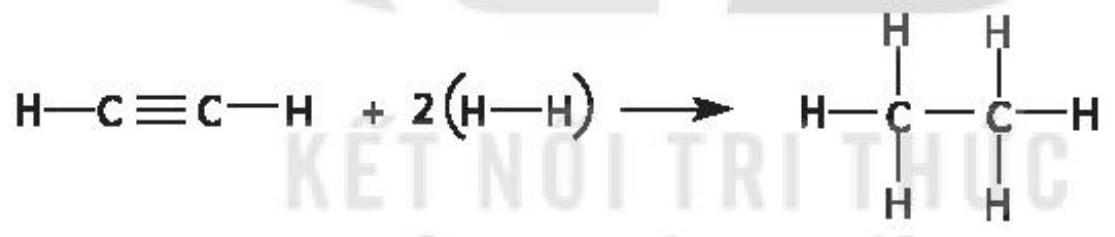
\includegraphics[max width=\textwidth, center]{2025_10_23_ee735750217b2aca435cg-41}

$$
\begin{aligned}
\Delta \mathrm{H} & =2 \mathrm{E}_{(\mathrm{C}-\mathrm{H})}+\mathrm{E}_{(\mathrm{C} \equiv \mathrm{C})}+2 \mathrm{E}_{(\mathrm{H}-\mathrm{H})}-6 \mathrm{E}_{(\mathrm{C}-\mathrm{H})}-\mathrm{E}_{(\mathrm{C}-\mathrm{C})} \\
& =(2 \cdot 414)+839+(2 \cdot 436)-(6 \cdot 414)-347=-292(\mathrm{~kJ} / \mathrm{mol})
\end{aligned}
$$

Phản ứng toả nhiệt.\\
18.17. a) Phản ứng (1) cần tiêu hao 1 nhiệt lượng để tách $\mathrm{SO}_{2}$ ra thành S và $\mathrm{O}_{2}$ nên toả nhiệt lượng ít hơn so với phản ứng (2).\\
b) $\Delta_{\mathrm{r}} \mathrm{H}_{298}^{\circ}(1)=2 \Delta_{\mathrm{f}} \mathrm{H}_{298}^{\circ}\left(\mathrm{H}_{2} \mathrm{O}\right)-2 \Delta_{\mathrm{f}} \mathrm{H}_{298}^{\circ}\left(\mathrm{H}_{2} \mathrm{~S}\right)-\Delta_{\mathrm{f}} \mathrm{H}_{298}^{\circ}\left(\mathrm{SO}_{2}\right)=-237(\mathrm{~kJ})$.

$$
\begin{aligned}
& \Delta_{\mathrm{r}} \mathrm{H}_{298}^{\mathrm{o}}(2)=2 \Delta_{\mathrm{f}} \mathrm{H}_{298}^{\mathrm{o}}\left(\mathrm{H}_{2} \mathrm{O}\right)-2 \Delta_{\mathrm{f}} \mathrm{H}_{298}^{\mathrm{o}}\left(\mathrm{H}_{2} \mathrm{~S}\right)=-530,5(\mathrm{~kJ}) . \\
& \Delta_{\mathrm{r}} \mathrm{H}_{298}^{\mathrm{o}}(2)-\Delta_{\mathrm{r}} \mathrm{H}_{298}^{\mathrm{o}}(1)=\Delta_{\mathrm{f}} \mathrm{H}_{298}^{\mathrm{o}}\left(\mathrm{SO}_{2}\right)=-530,5-(-237)=-293,5(\mathrm{~kJ}) .
\end{aligned}
$$

18.18. Phản ứng xảy ra:

$$
\mathrm{HCl}(\mathrm{aq})+\mathrm{NaHCO}_{3}(\mathrm{aq}) \rightarrow \mathrm{NaCl}(\mathrm{aq})+\mathrm{H}_{2} \mathrm{O}(\mathrm{l})+\mathrm{CO}_{2}(\mathrm{~g})
$$

$\Delta \mathrm{H}=(-407)+(-286)+(-392)-(-168)-(-932)=15(\mathrm{~kJ})$\\
$\Rightarrow$ Phản ứng thu nhiệt.\\
Số $\mathrm{mol} \mathrm{HCl}=$ số $\mathrm{mol} \mathrm{NaHCO}_{3}=0,1 \mathrm{~mol} \Rightarrow \mathrm{Q}=0,1 \cdot 15=1,5(\mathrm{~kJ})$.\\
Nhiệt độ giảm đi: $\Delta \mathrm{T}=\frac{1,5 \cdot 10^{3}}{200 \cdot 4,2}=1,8^{\circ} \mathrm{C}$.\\
$\Rightarrow$ Nhiệt độ cuối cùng là: $28-1,8=26,2^{\circ} \mathrm{C}$.\\
18.19. Khi trộn hai dung dịch, nhiệt độ trước phản ứng là: $\frac{25+26}{2}=25,5^{\circ} \mathrm{C}$.

Nhiệt lượng toả ra là:\\
$\mathrm{Q}=(50+50) \cdot 4,2 \cdot(28-25,5)=1050(\mathrm{~J})$.\\
Phản ứng xảy ra:

$$
\mathrm{AgNO}_{3}(\mathrm{aq})+\mathrm{NaCl}(\mathrm{aq}) \rightarrow \mathrm{AgCl}(\mathrm{~s})+\mathrm{NaNO}_{3}(\mathrm{aq})
$$

Số $\mathrm{mol} \mathrm{AgNO}_{3}=$ số $\mathrm{mol} \mathrm{NaCl}=\frac{0,5 \cdot 50}{1000}=0,025$.\\
$\Rightarrow \Delta \mathrm{H}=\frac{1050}{0,025}=42000 \mathrm{~J}=42(\mathrm{~kJ})$.\\
18.20. Gọi số $\mathrm{mol} \mathrm{CH}_{3} \mathrm{OH}$ và $\mathrm{C}_{2} \mathrm{H}_{5} \mathrm{OH}$ trong 10 g X lần lượt là a và b.

Ta có: $32 \mathrm{a}+46 \mathrm{~b}=10$\\
và $716 a+1370 b=291,9$

Giải hệ (I) và (II), ta được: $\mathrm{a}=0,025 ; \mathrm{b}=0,2$.\\
$\Rightarrow$ Khối lượng $\mathrm{CH}_{3} \mathrm{OH}$ là: $32 \cdot 0,025=0,8(\mathrm{~g})$.\\
$\Rightarrow$ Phần trăm tạp chất methanol trong X bằng $8 \%$.

\section*{CHUONG < 6 > TÓC ĐỘ PHẢN ÚNG}
\begin{table}[h]
\begin{center}
\captionsetup{labelformat=empty}
\caption{Bài 19. TỐC ĐỘ PHẢN ÚNG}
\begin{tabular}{|l|l|l|l|l|}
\hline
19.1. D & 19.2. A & 19.5. C & 19.6. D & 19.8. C \\
\hline
19.9. B & 19.10. A & 19.18. C & 19.25. D &  \\
\hline
\end{tabular}
\end{center}
\end{table}

19.3. a) (i) giảm (do HCl phản ứng với $\mathrm{Na}_{2} \mathrm{CO}_{3}$ làm nồng độ $\mathrm{Na}_{2} \mathrm{CO}_{3}$ giảm);\\
(ii) không thay đổi;\\
(iii) giảm (do làm giảm nồng độ $\mathrm{Na}_{2} \mathrm{CO}_{3}$ );\\
(iv) tăng (do $\mathrm{K}_{2} \mathrm{CO}_{3}$ cũng phản ứng với $\mathrm{CO}_{2}$ ).\\
b) Nếu tăng áp suất, tốc độ phản ứng tăng.\\
19.4. Tốc độ các phản ứng $\mathrm{a}, \mathrm{b}, \mathrm{c}, \mathrm{e}$ thay đổi khi áp suất thay đổi.\\
19.7. Đun nóng nước để phản ứng với magnesium nhanh hơn.\\
19.11. Các phản ứng xảy ra nhanh: (1), (3).

Các phản ứng xảy ra chậm: (2), (4).\\
19.12. Tốc độ trung bình của phản ứng hoà tan magnesium:

$$
\mathrm{v}=-\frac{0-0,1}{5}=0,02(\mathrm{~g} / \mathrm{s}) .
$$

19.13. Lượng zinc đã tan là: $0,4-0,05=0,35(\mathrm{~mol})$.

Thời gian để hoà $\tan 0,35 \mathrm{~mol}$ zinc là: $\frac{0,35}{0,005}=70(\mathrm{~s})$.\\
19.14. Tốc độ phản ứng trung bình:

$$
\mathrm{v}=-\frac{\Delta \mathrm{C}_{\mathrm{O}_{2}}}{3 \Delta \mathrm{t}}=-\frac{0,02-0,024}{3 \cdot 5}=2,67 \cdot 10^{-4}(\mathrm{~mol} /(\mathrm{L} \cdot \mathrm{~s})) .
$$

19.15. Tốc độ các phản ứng thay đổi khi thêm nước vào bình phản ứng:\\
a) Tăng (do nồng độ nước tăng).\\
b) Giảm (do nước làm loãng nồng độ $\mathrm{H}_{2} \mathrm{SO}_{4}$ ).\\
c) Giảm (do nước làm loãng nồng độ các chất tham gia phản ứng).\\
19.16. Phản ứng (1) có tốc độ cao hơn.\\
$\Rightarrow$ Phản ứng (1) đã sử dụng nồng độ HCl cao hơn.\\
19.17. a) $v=k \cdot C_{\mathrm{H}_{2} \mathrm{O}_{2}}$.\\
b) Theo thời gian, nồng độ $\mathrm{H}_{2} \mathrm{O}_{2}$ giảm dần nên tốc độ phản ứng giảm dần.\\
19.19. Nhiệt độ thấp, tốc độ phản ứng phân huỷ xảy ra rất chậm.\\
19.20. a) Hệ số nhiệt độ: $\gamma=\frac{4,5 \cdot 10^{-7}}{2 \cdot 10^{-7}}=2,25$.\\
b) Tốc độ phản ứng ở $60^{\circ} \mathrm{C}$ : $\mathrm{v}=\frac{2 \cdot 10^{-7}}{2,25}=8,89 \cdot 10^{-8}(\mathrm{~mol} /(\mathrm{L} . \mathrm{s}))$.\\
19.21. Đường kính có kích thước hạt nhỏ nên diện tích bề mặt lớn, phản ứng nhiệt phân tạo nước hàng nhanh chóng. Đường phèn có kích thước hạt lớn nên diện tích bề mặt lớn, khó phản ứng tạo nước hàng.\\
19.22. Dạng bột để tăng diện tích bề mặt tiếp xúc giữa xúc tác và $\mathrm{H}_{2} \mathrm{O}_{2}$.\\
19.23. Đập nhỏ đá vôi để tăng diện tích bề mặt, tăng tốc độ phản ứng phân huỷ. Tuy nhiên, nếu nghiền đá vôi thành bột mịn thì $\mathrm{CO}_{2}$ lại khó thoát ra khỏi khối chất rắn. Khi đó $\mathrm{CO}_{2}$ lại tác dụng với CaO ở nhiệt độ cao, tạo thành $\mathrm{CaCO}_{3}$ :

$$
\mathrm{CaO}+\mathrm{CO}_{2} \rightarrow \mathrm{CaCO}_{3}
$$

19.24. a) Biểu thức tính tốc độ phản ứng trung bình:

$$
\mathrm{v}=-\frac{\Delta \mathrm{C}_{\mathrm{NH}_{3}}}{4 \cdot \Delta \mathrm{t}}=-\frac{\Delta \mathrm{C}_{\mathrm{O}_{2}}}{5 \cdot \Delta \mathrm{t}}=\frac{\Delta \mathrm{C}_{\mathrm{NO}}}{4 \cdot \Delta \mathrm{t}}=\frac{\Delta \mathrm{C}_{\mathrm{H}_{2} \mathrm{O}}}{6 \cdot \Delta \mathrm{t}}
$$

b) Trong bình kín, tỉ lệ về nồng độ chính là tỉ lệ về số mol. Do đó, tốc độ phản ứng có thể được tính thông qua công thức:

$$
\mathrm{v}=-\frac{\Delta \mathrm{n}_{\mathrm{NH}_{3}}}{4 \cdot \Delta \mathrm{t}}=-\frac{\Delta \mathrm{n}_{\mathrm{O}_{2}}}{5 \cdot \Delta \mathrm{t}}=\frac{\Delta \mathrm{n}_{\mathrm{NO}}}{4 \cdot \Delta \mathrm{t}}=\frac{\Delta \mathrm{n}_{\mathrm{H}_{2} \mathrm{O}}}{6 \cdot \Delta \mathrm{t}}
$$

Ta có: $\mathrm{n}_{\mathrm{H}_{2} \mathrm{O}}=0,024 \mathrm{~mol}$.\\
Tốc độ trung bình của phản ứng: $\mathrm{v}=\frac{\mathrm{n}_{\mathrm{H}_{2} \mathrm{O}}}{6 \cdot \Delta \mathrm{t}}=\frac{0,024-0}{6 \cdot(2,5-0)}=1,6 \cdot 10^{-3}(\mathrm{~mol} / \mathrm{h})$.\\
c) Ta có: số $\mathrm{mol} \mathrm{NH}_{3}$ ban đầu là 0,025 ; số $\mathrm{mol} \mathrm{O}_{2}$ ban đầu là $0,03 \mathrm{~mol}$.

$$
\mathrm{v}=-\frac{\Delta \mathrm{n}_{\mathrm{NH}_{3}}}{4 \cdot \Delta \mathrm{t}}=-\frac{\Delta \mathrm{n}_{\mathrm{O}_{2}}}{5 \cdot \Delta \mathrm{t}}=1,6 \cdot 10^{-3}(\mathrm{~mol} / \mathrm{h})
$$

$\Rightarrow$ Sau 2,5 giờ, số $\mathrm{mol} \mathrm{NH}_{3}$ còn lại là $9.10^{-3} \mathrm{~mol}$; số $\mathrm{mol} \mathrm{O}_{2}$ còn lại là $0,01 \mathrm{~mol}$.\\
19.26. a) Đồ thị:\\
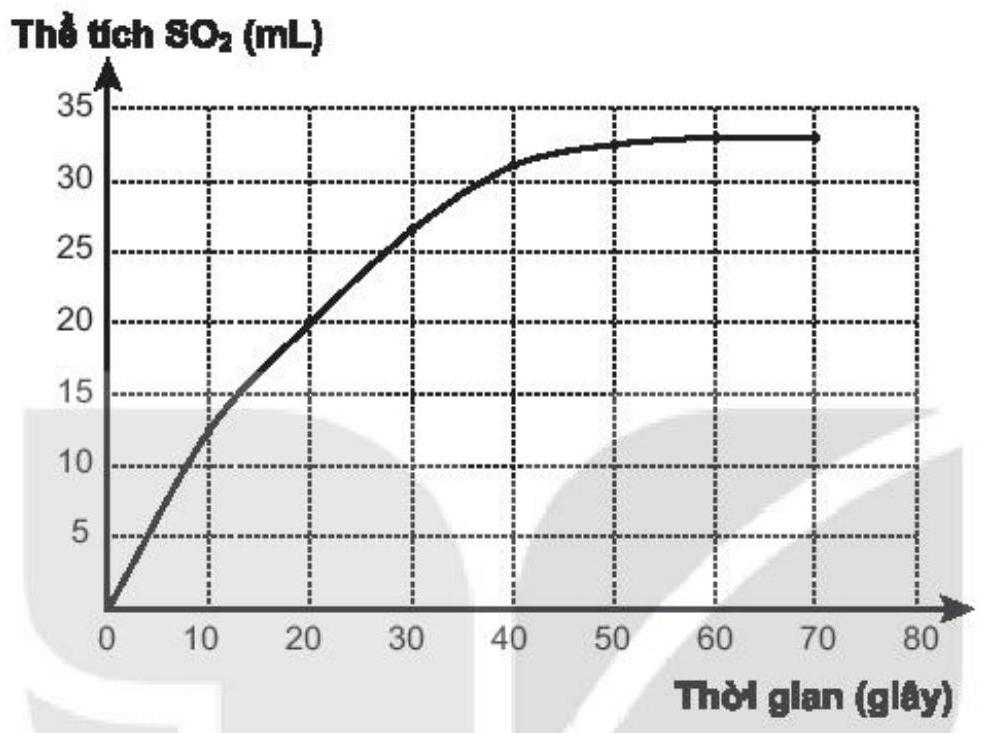
\includegraphics[max width=\textwidth, center]{2025_10_23_ee735750217b2aca435cg-45}\\
b) Thời điểm đầu: tốc độ phản ứng rất nhanh.\\
c) Thời điểm kết thúc phản ứng: đồ thị nằm ngang.\\
d) Tốc độ trung bình trong các khoảng thời gian:

\begin{itemize}
  \item Từ $0 \div 10$ giây: $v=\frac{12,5-0}{10-0}=1,25(\mathrm{~mL} / \mathrm{s})$;
  \item Từ $10 \div 20$ giây: $v=\frac{20,0-12,5}{20-10}=0,75(\mathrm{~mL} / \mathrm{s})$;
  \item Từ $20 \div 40$ giây: $v=\frac{31,0-20,0}{40-20}=0,55(\mathrm{~mL} / \mathrm{s})$.\\
19.27. Thay giá trị của v và nồng độ $\mathrm{ClO}_{2}, \mathrm{NaOH}$ lần lượt vào biểu thức tốc độ phản ứng.\\
$\Rightarrow \mathrm{x}=2$ và $\mathrm{y}=1$.\\
19.28. a) Đại lượng đo: nồng độ HBr thay đổi theo thời gian.
\end{itemize}

Đồ thị có dạng:\\
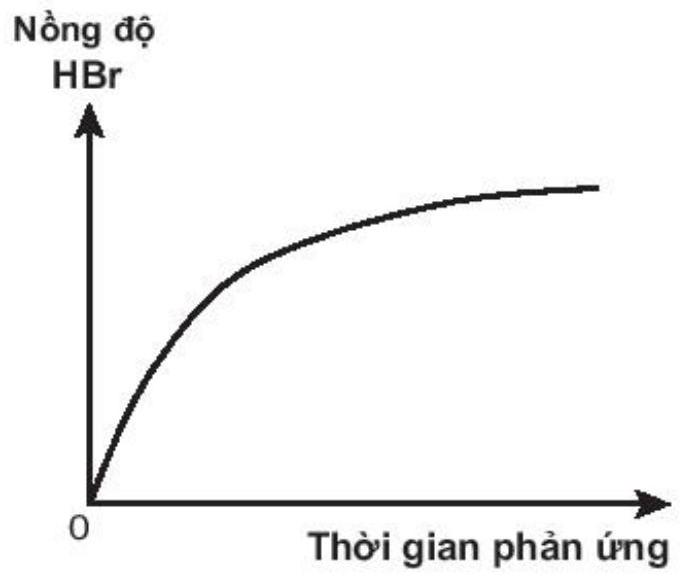
\includegraphics[max width=\textwidth, center]{2025_10_23_ee735750217b2aca435cg-46(1)}\\
(Nồng độ dung dịch HBr tăng dần theo thời gian. Khi phản ứng kết thúc, đường này nằm ngang).\\
b) Đại lượng đo: áp suất tổng cộng thay đổi theo thời gian.

Đồ thị có dạng:\\
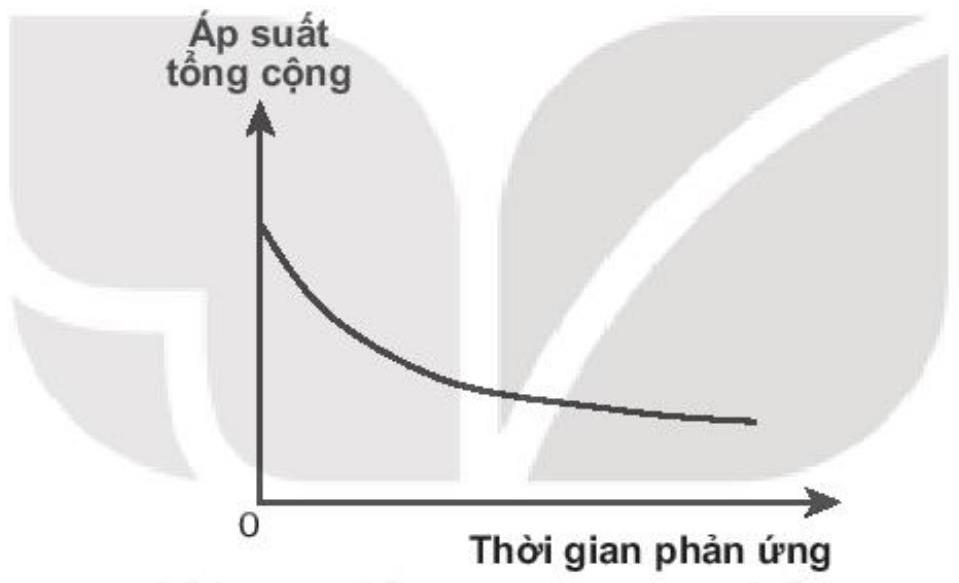
\includegraphics[max width=\textwidth, center]{2025_10_23_ee735750217b2aca435cg-46}\\
(Khi phản ứng xảy ra, số mol khí giảm nên áp suất tổng cộng giảm theo thời gian. Khi phản ứng kết thúc, đường này nằm ngang).\\
19.29. Đường (a): nồng độ HCl thay đổi theo thời gian (nồng độ tăng dần, lượng tăng gấp đôi $\mathrm{I}_{2}$ ).\\
Đường (b): nồng độ $\mathrm{I}_{2}$ thay đổi theo thời gian (nồng độ tăng dần).\\
Đường (c): nồng độ ICl thay đổi theo thời gian (nồng độ giảm dần, lượng giảm gấp đôi $\mathrm{H}_{2}$ ).\\
Đường (d): nồng độ $\mathrm{H}_{2}$ thay đổi theo thời gian (nồng độ giảm dần).\\
19.30. a) Tốc độ phản ứng tăng lên 2 lần.\\
b) Tốc độ phản ứng giảm 8 lần.\\
19.31. a) $7,5 \mathrm{~mL} / \mathrm{min}$.\\
b) $2,5 \mathrm{~min}$.\\
19.32. a) Tốc độ phản ứng ở $25^{\circ} \mathrm{C}$ là $0,27 \mathrm{~g} / \mathrm{min}$.

Tốc độ phản ứng ở $35^{\circ} \mathrm{C}$ là $0,57 \mathrm{~g} / \mathrm{min}$.\\
Hệ số nhiệt độ của phản ứng: $\gamma=\frac{0,57}{0,27}=2,11$.\\
b) Tốc độ phản ứng ở $45^{\circ} \mathrm{C}$ là $1,20 \mathrm{~g} / \mathrm{min}$.

Khối lượng cốc sau 1 phút là: $235,40-1,20=234,20(\mathrm{~g})$.\\
19.33. Miếng iron có nhiều lỗ có diện tích bề mặt lớn hơn nên lúc đầu tốc độ phản ứng với HCl cao hơn. Đồ thị (2) mô tả tốc độ thoát khí từ miếng iron B , Đồ thị (1) mô tả tốc độ thoát khí từ miếng iron A .\\
19.34. Xúc tác $\mathrm{MnO}_{2}$ có hiệu quả cao hơn vì đồ thị nồng độ $\mathrm{H}_{2} \mathrm{O}_{2}$ theo thời gian khi có mặt $\mathrm{MnO}_{2}$ dốc hơn khi có $\mathrm{Fe}_{2} \mathrm{O}_{3}$.\\
19.35. a) Tia lửa điện chỉ cung cấp năng lượng, không là chất xúc tác. Phân tử $\mathrm{H}_{2}$ và $\mathrm{O}_{2}$ hấp thụ năng lượng đó để có năng lượng cao hơn giá trị năng lượng hoạt hoá, xảy ra phản ứng.\\
Chư ý: Nhiệt tạo thành ra từ phản ứng $\mathrm{H}_{2}+\mathrm{O}_{2} \rightarrow 2 \mathrm{H}_{2} \mathrm{O}$ lại cung cấp năng lượng để phản ứng tiếp tục xảy ra.\\
b) Bột kim loại là chất xúc tác, làm giảm năng lượng hoạt hoá của phản ứng, giúp phản úng xảy ra.

\begin{table}[h]
\begin{center}
\captionsetup{labelformat=empty}
\caption{Bài 20. ÔN TẬP CHƯƠNG 6}
\begin{tabular}{|l|l|l|l|}
\hline
20.1. C & 20.3. C & 20.4. A & 20.5. C \\
\hline
\end{tabular}
\end{center}
\end{table}

20.2. Có thể dùng 3 cách:

\begin{itemize}
  \item Tăng nhiệt độ: đun nóng bình phản ứng.
  \item Tăng nồng độ: dùng dung dịch HCl đặc.
  \item Tăng diện tích bề mặt: dùng zinc (dạng bột) hoặc zinc có kích thước hạt nhỏ.\\
20.3. Các biện pháp làm tăng tốc độ phản ứng là (1), (2), (4), (5) (chọn C ).\\
20.6. a) Tốc độ phản ứng tỉ lệ nghịch với thời gian. Vậy khi tăng nhiệt độ từ $0^{\circ} \mathrm{C}$ lên $30^{\circ} \mathrm{C}$, tốc độ phản ứng tăng 8 lần.\\
Gọi hệ số nhiệt độlà $\gamma$, ta có: $\gamma^{\frac{30-0}{10}}=\frac{24}{3} \Rightarrow \gamma=2$.\\
b) Nếu bảo quản ở $20^{\circ} \mathrm{C}$, táo bị hư sau 6 ngày.\\
20.7. (1) Sai: các hạt (phân tử, nguyên tử, ion) của chất phản ứng phải va chạm với nhau và va chạm phải đủ mạnh mới gây ra phản ứng.\\
(2) Đúng.\\
(3) Sai: tốc độ phản ứng tăng lên bao nhiêu lần tuỳ thuộc vào hệ số nhiệt độ $\gamma$.\\
(4) Sai: năng lượng va chạm giữa hai phân tử chất phản ứng phải cao hơn năng lượng hoạt hoá để gây ra phản ứng.\\
(5) Đúng.\\
20.8. (i) Tốc độ phản ứng tăng lên 4 lần; (ii) Tốc độ phản ứng giảm đi 3 lần; (iii) Tốc độ phản ứng không đổi.\\
20.9. a) Hằng số tốc độ tỉ lệ thuận với tốc độ phản ứng.
\end{itemize}

Gọi hệ số nhiệt độ là $\gamma$, ta có: $\gamma^{\frac{227-127}{10}}=\frac{4,25 \cdot 10^{-4}}{1,60 \cdot 10^{-7}}$.\\
$\Rightarrow \gamma^{10}=2656,25 \Rightarrow \gamma=2,2$.\\
b) Gọi hằng số tốc độ ở $167^{\circ} \mathrm{C}$ là k . Ta có: $\gamma^{\frac{167-127}{10}}=\frac{\mathrm{k}}{1,60 \cdot 10^{-7}}$.

Thay $\gamma=2,2 \Rightarrow \mathrm{k}=3,75 \cdot 10^{-6}$.\\
20.10. a) Tốc độ phản ứng tỉ lệ nghịch với thời gian.

Gọi hệ số nhiệt độ là $\gamma$, ta có: $\gamma=\frac{3,8}{3,2}=1,1875$\\
b) Nếu luộc miếng thịt ở $80^{\circ} \mathrm{C}$, thời gian cần là: $3,8 \cdot 1,1875=4,5(\mathrm{~min})$.\\
20.11. Từ $0,128 \cdot 10^{-3} \mathrm{~g}$ dioxin phân huỷ còn lại $10^{-6} \mathrm{~g}$ tức là đã giảm:\\
$\frac{0,128 \cdot 10^{-3}}{10^{-6}}=128=2^{7}$ (lần).\\
Vậy thời gian cần thiết để $0,128 \cdot 10^{-3} \mathrm{~g}$ dioxin phân huỷ còn lại $10^{-6} \mathrm{~g}$ là:\\
$8 \cdot 7=56$ (năm).\\
20.12. a) Tốc độ phản ứng tỉ lệ nghịch với thời gian.

Vậy khi nhiệt độ tăng lên $10^{\circ} \mathrm{C}$ (từ $27^{\circ} \mathrm{C}$ lên $37^{\circ} \mathrm{C}$ ), thời gian để lượng hoạt chất giảm đi một nửa là: $\frac{10}{2,5}=4(\mathrm{~h})$.\\
b) Khi chất kháng sinh này chỉ còn $12,5 \%$ so với ban đầu, tức là lượng đã giảm $\frac{100}{12,5}=8=2^{3}$ (lần) so với ban đầu.\\
Thời gian cần để lượng chất kháng sinh giảm đi 8 lần là: $4 \cdot 3=12$ (h).

\section*{Bài 21. NHÓM HALOGEN}
\begin{center}
\begin{tabular}{|l|l|l|l|l|}
\hline
21.1. B & 21.2. D & 21.3. D & 21.4. C & 21.5. A \\
\hline
21.6. B & $21.7 . \mathrm{C}$ & $21.8 . \mathrm{A}$ & $21.9 . \mathrm{D}$ & $21.10 . \mathrm{B}$ \\
\hline
21.11. D & $21.12 . \mathrm{D}$ & $21.13 . \mathrm{C}$ & $21.14 . \mathrm{D}$ & $21.15 . \mathrm{B}$ \\
\hline
21.16. A & $21.17 . \mathrm{B}$ & $21.18 . \mathrm{B}$ & $21.19 . \mathrm{C}$ & $21.20 . \mathrm{B}$ \\
\hline
\end{tabular}
\end{center}

21.21. $\mathrm{F}_{2}$ tác dụng với $\mathrm{H}_{2}$ mạnh nhất nên phản ứng:

$$
\mathrm{H}_{2}(\mathrm{~g})+\mathrm{F}_{2}(\mathrm{~g}) \longrightarrow 2 \mathrm{HF}(\mathrm{~g})
$$

có biến thiên enthalpy âm nhất.\\
$\mathrm{I}_{2}$ tác dụng với $\mathrm{H}_{2}$ yếu nhất nên phản ứng:

$$
\mathrm{H}_{2}(\mathrm{~g})+\mathrm{I}_{2}(\mathrm{~g}) \longrightarrow 2 \mathrm{HI}(\mathrm{~g})
$$

có biến thiên enthalpy ít âm nhất.\\
Như vậy, biến thiên enthalpy của các phản ứng tăng dần trong dãy trên.\\
21.22. Áp dụng định luật bảo toàn khối lượng, ta có:

$$
\mathrm{m}_{\mathrm{Cl}_{2}}=1,332-0,48=0,852(\mathrm{~g}) \Rightarrow \mathrm{n}_{\mathrm{Cl}_{2}}=\frac{0,852}{71}=0,012(\mathrm{~mol})
$$

Phương trình hoá học:

$$
\mathrm{M}+\mathrm{Cl}_{2} \xrightarrow{\mathrm{t}^{\circ}} \mathrm{MCl}_{2}
$$

Mol: $0,012 \leftarrow 0,012$

$$
\mathrm{M}=\frac{0,48}{0,012}=40 . \mathrm{M} \text { là } \mathrm{Ca} .
$$

21.23. a) Phương trình hoá học:

\begin{center}
\begin{tabular}{lcll}
 & $\mathrm{H}_{2}+\mathrm{Cl}_{2}$ & $\longrightarrow 2 \mathrm{HCl}$ \\
Ban đầu (mol): & $0,04 \quad 0,04$ &  \\
Phản ứng (mol): & $0,036 \quad 0,036$ & $\leftarrow 0,072$ \\
\end{tabular}
\end{center}

Hiệu suất phản ứng là:\\
$\mathrm{H}=\frac{0,036}{0,04} \cdot 100 \%=90 \%$.\\
b) Phản ứng có số mol khí hai vế bằng nhau nên tổng số mol khí trước và sau phản ứng bằng nhau, dẫn tới áp suất bằng nhau: $\mathrm{P}_{1}=\mathrm{P}_{2}$.\\
21.24. Hiện tượng hồ tinh bột chuyển màu xanh tím chứng tỏ sau phản ứng ống thứ hai có sinh ra $\mathrm{I}_{2}$ nên muối X là KI .\\
Phương trình hoá học của các phản ứng:

$$
\begin{aligned}
& \mathrm{KI}+\mathrm{AgNO}_{3} \longrightarrow \mathrm{KNO}_{3}+\mathrm{AgI} \downarrow \\
& 2 \mathrm{KI}+\mathrm{Br}_{2} \longrightarrow 2 \mathrm{KBr}+\mathrm{I}_{2}
\end{aligned}
$$

21.25. a) Dung dịch hút ẩm cần có khả năng hút nước và không tác dụng với chất cần làm khô là $\mathrm{Cl}_{2}$, do vậy không chọn dung dịch có tính kiềm. Đề xuất chọn dung dịch $\mathrm{H}_{2} \mathrm{SO}_{4}$ đặc.\\
b) Để hạn chế khí $\mathrm{Cl}_{2}$ bay ra cần chọn dung dịch có tính kiềm để tẩm vào bông đậy ở miệng bình thu khí. Đề xuất chọn dung dịch $\mathrm{NaOH} 4 \%$.

\section*{Bài 22. HYDROGEN HALIDE. MUỐI HALIDE}
\begin{center}
\begin{tabular}{|l|l|l|l|l|}
\hline
22.1. C & $22.2 . \mathrm{C}$ & $22.3 . \mathrm{B}$ & $22.4 . \mathrm{A}$ & $22.5 . \mathrm{B}$ \\
\hline
22.6. D & $22.7 . \mathrm{D}$ & $22.8 . \mathrm{A}$ & $22.9 . \mathrm{C}$ & $22.10 . \mathrm{B}$ \\
\hline
22.11. A & $22.12 . \mathrm{C}$ & $22.13 . \mathrm{D}$ & $22.14 . \mathrm{B}$ & $22.15 . \mathrm{C}$ \\
\hline
$22.16 . \mathrm{A}$ & $22.17 . \mathrm{D}$ & $22.18 . \mathrm{C}$ & $22.19 . \mathrm{D}$ & $22.20 . \mathrm{C}$ \\
\hline
\end{tabular}
\end{center}

22.21. a) Hiện tượng nước phun vào bình chứng tỏ áp suất khí trong bình đã giảm rất nhanh.\\
b) Sự giảm nhanh áp suất chứng tỏ khí hydrogen chloride đă tan nhanh vào nước.\\
22.22. a) $\mathrm{NaHCO}_{3}+\mathrm{HCl} \longrightarrow \mathrm{NaCl}+\mathrm{CO}_{2}+\mathrm{H}_{2} \mathrm{O}$\\
b) $\left(\mathrm{C}_{6} \mathrm{H}_{10} \mathrm{O}_{5}\right)_{\mathrm{n}}+\mathrm{nH}_{2} \mathrm{O} \xrightarrow[\mathrm{t}^{\circ}]{\mathrm{HCl}} \mathrm{nC}_{6} \mathrm{H}_{12} \mathrm{O}_{6}$\\
22.23. $\mathrm{NaBr}+\mathrm{AgNO}_{3} \longrightarrow \mathrm{NaNO}_{3}+\mathrm{AgBr} \downarrow$ (màu vàng nhạt)

$$
2 \mathrm{NaBr}+\mathrm{Cl}_{2} \longrightarrow 2 \mathrm{NaCl}+\mathrm{Br}_{2}
$$

$\left(\mathrm{Br}_{2} \tan\right.$ vào trong benzene làm xuất hiện màu da cam).\\
22.24. X làm hồ tinh bột chuyển sang màu xanh tím nên X là dung dịch iodine. Z tác dụng với $\mathrm{NaHCO}_{3}$ tạo bọt khí nên Z là hydrochloric acid:

$$
\mathrm{NaHCO}_{3}+\mathrm{HCl} \longrightarrow \mathrm{NaCl}+\mathrm{CO}_{2}+\mathrm{H}_{2} \mathrm{O}
$$

Y là sodium chloride (chọn A ).

\begin{table}[h]
\begin{center}
\captionsetup{labelformat=empty}
\caption{Bài 23. ÔN TẬP CHƯƠNG 7}
\begin{tabular}{|l|l|l|l|l|l|}
\hline
23.1. A & $23.2 . \mathrm{C}$ & $23.3 . \mathrm{B}$ & $23.4 . \mathrm{A}$ & $23.5 . \mathrm{D}$ & $23.6 . \mathrm{C}$ \\
\hline
23.7. C & $23.8 . \mathrm{D}$ & $23.9 . \mathrm{B}$ & $23.10 . \mathrm{A}$ & $23.11 . \mathrm{D}$ & $23.12 . \mathrm{B}$ \\
\hline
23.13. D & $23.14 . \mathrm{A}$ & $23.15 . \mathrm{D}$ & $23.16 . \mathrm{C}$ & $23.17 . \mathrm{D}$ & $23.18 . \mathrm{C}$ \\
\hline
23.19. A & $23.20 . \mathrm{D}$ & $23.22 . \mathrm{C}$ &  &  &  \\
\hline
\end{tabular}
\end{center}
\end{table}

23.20. Chloramine-B ( $\mathrm{C}_{6} \mathrm{H}_{6} \mathrm{O}_{2} \mathrm{SNCl}$ ) là hợp chât hữu cơ chứa nguyên tử chlorine, dễ tác dựng với nước tạo thành hypocholrite có tác dụng diệt khuẩn mạnh: $\mathrm{C}_{6} \mathrm{H}_{6} \mathrm{O}_{2} \mathrm{SNCl}+\mathrm{H}_{2} \mathrm{O} \longrightarrow \mathrm{C}_{6} \mathrm{H}_{6} \mathrm{O}_{2} \mathrm{SNH}+\mathrm{HClO}$\\
23.21

$$
\begin{aligned}
& \mathrm{Cu}(\mathrm{OH})_{2}+2 \mathrm{HCl} \longrightarrow \mathrm{CuCl}_{2}+2 \mathrm{H}_{2} \mathrm{O} \\
& \mathrm{CuCO}_{3}+2 \mathrm{HCl} \longrightarrow \mathrm{CuCl}_{2}+\mathrm{CO}_{2}+2 \mathrm{H}_{2} \mathrm{O}
\end{aligned}
$$

23.22. Y hoà tan được silicon dioxide nên Y là dung dịch HF :

$$
\mathrm{SiO}_{2}+4 \mathrm{HF} \longrightarrow \mathrm{SiF}_{4}+2 \mathrm{H}_{2} \mathrm{O}
$$

Z tác dụng với dung dịch silver nitrate thu được kết tủa vàng nên Z là potassium iodide: $\mathrm{KI}+\mathrm{AgNO}_{3} \longrightarrow \mathrm{KNO}_{3}+\mathrm{AgI} \downarrow$

X là dung dịch hydrofluoric acid (chọn C ).\\
23.23. $\mathrm{n}_{\mathrm{NaCl}}=10 \cdot \frac{1,17}{100 \cdot 58,5}=0,002(\mathrm{~mol})$.

Thí nghiệm chỉ xảy ra phản ứng tạo kết tủa AgCl (lưuý AgF là muối tan):

$$
\begin{array}{rlr}
\mathrm{NaCl}+\mathrm{AgNO}_{3} & \longrightarrow \mathrm{NaNO}_{3}+\underset{0,002}{\mathrm{AgCl} \downarrow} \\
\text { Mol: } 0,002 & \rightarrow & 0,02
\end{array}
$$

$\mathrm{m}=0,002 \cdot 143,5=0,287(\mathrm{~g})$.\\
23.24. Phản ứng điện phân sinh ra khí chlorine ở anode, hydrogen và sodium hydroxide ở cathode: $2 \mathrm{NaCl}+2 \mathrm{H}_{2} \mathrm{O} \xrightarrow{\text { dpdd }} 2 \mathrm{NaOH}+\mathrm{H}_{2}+\mathrm{Cl}_{2}$

Do không có màng ngăn điện cực nên khí $\mathrm{Cl}_{2}$ và NaOH khuếch tán sang nhau trong bình điện phân và xảy ra phản ứng:

$$
2 \mathrm{NaOH}+\mathrm{Cl}_{2} \longrightarrow \mathrm{NaCl}+\mathrm{NaClO}+\mathrm{H}_{2} \mathrm{O}
$$

Tổng hợp hai phản ứng xảy ra trong quá trình điện phân là:

$$
\mathrm{NaCl}+\mathrm{H}_{2} \mathrm{O} \xrightarrow{\text { dpdd }} \mathrm{NaClO}+\mathrm{H}_{2}
$$

\section*{KẼT NỐI TRI THỨC \\
 Vớl CUỘC SỐNG}

\end{document}